\documentclass[draftclsnofoot,onecolumn]{IEEEtran}

\newcommand{\namesigdate}[2][5cm]{%
  \begin{tabular}{@{}p{#1}@{}}
    #2 \\[2\normalbaselineskip] \hrule \\[0pt]
    {\small \textit{Signature}} \\[2\normalbaselineskip] \hrule \\[0pt]
    {\small \textit{Date}}
  \end{tabular}
}

\usepackage[T1]{fontenc}
\usepackage[letterpaper, portrait, margin=0.75in]{geometry}
\usepackage{url}
\usepackage{listings}
\usepackage{color}
\usepackage{hyperref}
\setlength{\parindent}{0pt}
\usepackage{pgfgantt}
\usepackage{graphicx}

\begin{document}
\title {Final Report for Noctilucent VR}
\author {Taylor Fahlman, Joshua Bowen, Adam Puckette}

\maketitle

\abstract
Lidar is a powerful piece of technology that has been used for several years to map large real life locations to scale, for disaster relief, surveying, and other important geomatics problems.
In an effort to improve the use of this technology we have worked to create a Virtual Reality extension to the open-source cloud viewing software potree Viewer.
In this document you will find a years worth of effort and research into the capabilities a possibilities of Virtual Reality with Lidar Technology.
It is our hope that this document will serve as a guide and a tool to those seeking to pick up where we left off in pursuing Virtual Reality Point-Cloud Data.

\newpage
\section{Introduction}

Noctilucent VR is a WebVR-based plugin for the point-cloud viewing application, potree Viewer. 
This plugin adds a virtual reality (VR) mode to the application which can be activated at the press of a button. 
The VR mode renders the point cloud in a 3D stereoscopic display suitable for VR headsets such as the Google Cardboard. 
This project was proposed by Matt O'Banion of the Geomatics laboratory at OSU in order to explore a cheaper, more portable and accessible alternative to their existing 3D TV setup. 
Mr. O'Banion also wished to experiment with the immersive aspects of a virtual-reality headset in the pursuit of his work with point cloud data sets. 
The potential of this project is in its accessible and inexpensive nature. 
With ready access to point-cloud data through the internet, anyone with a reasonably powerful computer and compatible VR headset could view point-cloud data in a more immersive format. 

The Noctilucent VR team consists of Joshua Bowen, Adam Puckette, and Taylor Fahlman. 
We divided up into unofficial roles over course of the past year, with each of us taking on different responsibilities. 
Joshua was our team captain, coordinating with our client and the university, while Taylor focused on the code and other technical sides of the project. 
Adam dealt mainly with research into OSVR and point-cloud viewing software, as well as documentation.
Our client was quite involved in the project, directing our efforts and pointing towards the resources we would need. 
He took the role of director and supervisor over the course of the term, and worked directly with us to make Noctilucent VR what it is.

\clearpage
\section{Requirements Document}

\documentclass{article}

\newcommand{\namesigdate}[2][5cm]{%
  \begin{tabular}{@{}p{#1}@{}}
    #2 \\[2\normalbaselineskip] \hrule \\[0pt]
    {\small \textit{Signature}} \\[2\normalbaselineskip] \hrule \\[0pt]
    {\small \textit{Date}}
  \end{tabular}
}

\usepackage[T1]{fontenc}
\usepackage[letterpaper, portrait, margin=0.75in]{geometry}
\usepackage[singlespacing]{setspace}
\usepackage{url}
\usepackage{tocloft}
\usepackage{listings}
\usepackage{color}
\usepackage{pgfgantt}
\setlength{\parindent}{0pt}

\begin{document}
\title {Requirements for Noctilucent VR}
\author {Taylor Fahlman, Joshua Bowen, Adam Puckette}

\maketitle

\abstract
There are 4 main deliverables for this project. Creating an OpenGL test for the OSVR framework;
writing a proposal to either use CloudCompare or another software; a simple documentation/summary of
the final product; and the final product, where an OSVR headset can interact with the software.

\newpage
\thispagestyle{empty}
\mbox{}

\section{Introduction}
\subsection{Purpose}

The purpose of this addon is to allow any user of the open source software CloudCompare to be able to view point cloud data in Virtual Reality.
The user, however, must be in possession of some Virtual Reality headset.
In this regard this project is designed for anyone who utilizes CloudCompare for it's open source cloud data viewing capabilities,
and is looking for a more immersive analysis of data.

\subsection{Scope}

Noctilucent VR will function as an extension or addon of the already existent open source software CloudCompare.
When utilized, the software will take the point cloud data as rendered by CloudCompare and display it in a fashion suitable for virtual reality.
The software will render and update the display of the data in at least 30 Frames Per Second at a consistent rate.
An Auxillery device will also be useable to navigate the data.
Benefits of the software include the viewing of point cloud data in a more immersive enviroment.
While viewing the data the software should not freeze or stutter and should draw complete scenes. 
Additionally the software must render at least a million point, ideally more.
As point cloud data often contain millions of points it is important that this software is able to render as many points as possible.

\subsection{Definitions}

Free and Open Source Software: Also known as FOSS, is any software that can be classified as both free software and open source software. This means that anyone is freely licensed to modify, copy, or study the code as they see fit. 
Users are encouraged to improve the software and share their work with others.

Virtual Reality: Also referred to as VR, is an existing technology which allows the user to put on a headset and have an immersive experience in which turning your head turns the camera and moving your head moves the camera.
Additionally, visuals are rendered seperatly for both eyes allowing for different perspectives which when put together create a 3D steroscopic environment.

CloudCompare: Also referred to as CC, is a FOSS program freely available to users who need to view and analyze point cloud data.

Open Source Virtual Reality: Also referred to as OSVR, is an existing Open Source VR headset and VR software platform. OSVR is designed so that it can be developed on and modified by the the public at only the cost of the headwear.

Oculus Developers Kit 2: Also called the DK2, is another existing VR headset, however it is not open source and has since been replaced with a standard production model.

Graphics Processing Unit: Referred to as a GPU, is the piece of hardware inside of a computer responsible for performing microprocesses often associated with graphics rendering or deep learning.

Frames Per Second: Called FPS, is the refresh rate at which the computer draws a scene over the course of a second.

\subsection{References}

The following links are our references:
  http://www.danielgm.net/cc/
  http://www.osvr.org/

\subsection{Overview}

The user of selected software will be able to plug in an OSVR-supported headset and view their point cloud data in a 3D VR view.
They will be able to examine and manipulate the data in 3D space. 
They will be able to rotate and zoom, crop, etc. large data sets at a frame rate of at least 30 FPS with a stable FPS.
A stable FPS is an FPS that is within plus or minus 5 FPS of the average FPS over a 5 second period.
The software should not freeze for longer than half a second more than 3 times over 5 seconds.
Additionally, freezes longer than 2 seconds at any point must be avoided.
All renderings should not experience screen tearing more than once every 3 seconds.
At least a million points of cloud data must be able to be rendered while meeting all these requirements.

\section{Overall Desciption}
\subsection{Product Perspective}

\subsubsection{User Interfaces}

Noctilucent VR will make a mild modification to the current CloudCompare interface by adding an option to activate VR mode. 
When activated CC will begin rendering data for VR instead of for a monitor.
When in VR mode, CC will utilize a different interace from the default version.
The new user interface will be designed with VR in mind and will only appear at the need of the user upon the push of a button.
The VR Interface will include functionality to easily navigate the data and mark areas of interest.

\subsubsection{Hardware Interfaces}

Noctilucent VR will interface with the GPU of the computer to render graphics.
The software will also utilizie some VR Headset, with the main target being the
OSVR Headset, and the Oculus Rift Headset as a secondary goal.

\subsubsection{Software Interfaces}

Name: CloudCompare
Mnemonic: CC
Specification Number:
Version Number: 2.7
Source.

CloudCompare will be the software that handles the actual analysis and input of the cloud data information. 
In relation to our software product we will take what exists already with CloudCompare and add the ability for the software to render the data for VR.

\subsection{Product Functions}

Noctilucent VRs Functions are as follows

%\item Render point cloud data in virtual reality
%\item Provide an interface to interact with data
\begin{enumerate}
\item Render point cloud data in virtual reality
\item Provide an interface to interact with data
\end{enumerate}

\subsection{User Characteristics}

Someone using this software is expected to already be familiar with point cloud data and softwares used to navigate it. 
Familiarity with CloudCompare is expected before jumping into the VR aspects of it.
This might be a users first experience with VR if they purchased it for this purpose.

\subsection{Constraints}

The possible constraints mostly rely in the way CC uses OpenGL. There have been repoted issues with the software in which
stuttering was found with larger data sets. With this possible limitation already present in 2D view, enabling 3D support would
likely make the situation worse. However, the lead developer has stated he will help in this case, and some of these problems 
may be able to be fixed. In the case that theses cannot be fixed, there is also a linux-only research program which can be used
instead that already supports 3D steroscopic viewing.

\subsection{Assumptions and Dependencies}

It is our assumption that CC will be capable of rendering a million or more points of cloud data in realtime.
In the event that CC is not capable of such we will need to considering creating a seperate software instead of an extension.

\section{Specific Requirements}

Specifically, an OpenGL program written to test the OSVR framework will be needed. This will simply involve an OBJ viewer in OpenGL,
and some 3D OBJ file to view. 

Reasearch will be needed on the constraints of OpenGL. Specifically, the viability of CC as the medium of delivery will need to be
assesed. A comparison against the research linux-based software will be included in this reasearch.

Once a solution is decided on, documentation of the implementation will be written. This will address what parts of
the architechture was needed to implement this change, as well as setting and other relevant information for future developers
and users of the final product. 

Finally, either a plugin or change to the core code will need to be written and presented to the client, as well as the reposity or
stakeholder of the software we choose. The ideal situation is that the finally product would be integrated into the core of the 
software. However, an external plugin would suffice. 

\newpage
%Gantt chart
\begin{ganttchart}[
        hgrid=true,
        vgrid={*{10}{blue, dashed}},
        y unit chart=0.75cm,
        x unit=0.75cm
    ]{1}{13}
    \gantttitle{Senior Project 2016-2017}{13} \\
    \gantttitlelist{4, 6, 8, 10, 2, 4, 6, 8, 10, 2, 4, 6, 8}{1} \\
    \ganttgroup{Documentation}{1}{4}\\
    \ganttbar[progress=100]{Problem Statemenet}{1}{2}\\
    \ganttbar[progress=50]{Requirements Document}{1}{3}\\
    \ganttbar[progress=0]{Technical Review}{2}{4}\\
    \ganttbar[progress=0]{Design Document}{2}{4}\\
    \ganttgroup{Implementation}{1}{12}\\
    \ganttbar[progress=0]{OpenGL OSVR Harness}{1}{4}\\
    \ganttbar[progress=0]{Research on Software}{4}{7}\\
    \ganttbar[progress=0]{Documentation}{7}{12}\\
    \ganttbar[progress=0]{Integration of OSVR and Software}{7}{12}\\
    \ganttgroup{Presentation}{8}{13}\\
    \ganttbar[progress=0]{Presentation Board}{10}{13}\\
    \ganttbar[progress=0]{Expo Setup}{10}{13}\\
\end{ganttchart}
\newpage
\vspace{2pc}

\noindent \namesigdate{Matt O'Banion} \hfill \namesigdate[3cm]{Adam Puckette}

\vspace{2pc}

\noindent \namesigdate{Taylor Fahlman} \hfill \namesigdate[3cm]{Joshua Bowen}

\end{document}



\section{Requirements Document Changes}

\begin{table}[ht]
\caption{Changes in the Requirements Document}
\centering
\begin{tabular}{l l l}
\hline
\hline
    Requirements & What Changed & Comments \\
    \hline
    OpenGL Deliverable & Project shifted from OpenGL to WebGL & We had a WebGL demo, but it wasn't requested by our client so it is not part of the final documentation \\
    Proposal of Software & Discussed informally with client and made decision without a write-up & Due to the nature of our project, our client decided to change software without needing a formal proposal\\
    Use of CloudCompare & Client requested a move to potree due to time and ease of use & This move was beneficial to the project and we wish we had made the move sooner.\\
    Manipulate data with zoom, rotate, crop, etc. & Due to the change to potree, some of the analysis tools were no longer available to us & This is something that would need to be added to potree before it can be added to our project.
    
\end{tabular}
\end{table}
\newpage

\section{Design Document}

\title {Design Document for Noctilucent VR}
\author {Taylor Fahlman, Joshua Bowen, Adam Puckette}

\maketitle

\abstract

Noctilucent VR will allow users to view and manipulate point-cloud data in virtual reality. 
The required concepts, terminologies, design viewpoints, and use methodologies for Noctilucent VR are described herein. 
ctilucent VR will be created by integrating an existing open source point-cloud viewing program with the OSVR framework. 
This will allow us to create modular and platform-independent software. 
With Noctilucent VR, anyone with a virtual reality headset will be able to download and view point-cloud data without needing specialized hardware.

\subsection{Overview}
\subsubsection{Scope}

This document describes the software design and information regarding the Virtual Reality Lidar Point Cloud Viewing Software known as Noctilucent VR.
This software is intended to be used by professionals seeking to improve their Lidar Cloud viewing experience.
Uses can include anything from casual cloud data viewing to professional informatics.

Noctilucent and it's design can be used on any computer capable of handling the graphics rendering.
This projects only applicability restriction is in the capabilities of the computer running it.

\subsubsection{Purpose}

Noctilucent VR exists to expand the current capabilities of humans to view Lidar Cloud data.
Specifically the goal of this project is to take 3D information previously displayed in 2D and provide an easy to use, easily accessible, Open Source alternative to viewing this data which allows for it's viewing in 3D.
This project exists as viewing 3D data in 3D is an important aspect of being able to garner easily all the information from that data as possible.

\subsubsection{Intended Audience}

This project is primarily intended to be used by scientists, engineers, and those who perform informatics, however, the project is not limited to those audiences.
The Free and Open Source nature of this project allows it's use by anyone with access to cloud compare, a virtual reality headset, a wiimote, and a computer capable of running this software.

\subsubsection{Conformance}

Noctilucent VR conforms to this document if it satisfies the requirements as they are outlined in subsections 4 and 5 of this Document. Requirements are denoted by the verb shall.

\subsection{Definitions}

{\parindent0pt
\textbf{Free and Open Source Software (FOSS)}\\

Any software that can be classified as both free software and open source software.
This means that anyone is freely licensed to modify, copy, or stufy the code as they see fit.
Users are encouraged to improve the software and share their work with others.\\

\textbf{Virtual Reality (VR)}\\

An Existing technology which allows the user to put ona headset and have an immersive experience in which turning your  head turns the camera and mmoving your head moves the camera.
Visuals are rendered seperately for both eyes allowing for different perspectives which come together to create a 3D stereoscopic environment.\\

\textbf{CloudCompare (CC)}\\

A FOSS program freely available to users who need to view and analyze point cloud data.\\

\textbf{Open Source Virtual Reality (OSVR)}\\

An existing Open Source VR Headset and VR Software platform.
OSVR is designed so that it can be developed on and modified by the public at only the cost of the headwear.\\

\textbf{Graphics Processing Unit (GPU)}\\

The piece of hardware inside a computer responsible for performing microprosses often associated with graphics rendering or deep learning.\\

\textbf{Frames Per Second (FPS)}\\

The refresh rate at which the computer draws a scene over the course of a second.\\
}

\subsection{Design}

\subsubsection{Stakeholders}

Matt O'Banion - For use in geo-informatics

\subsubsection{Design Concerns}

\begin{itemize}
 \item Shall have a user interface for interacting with the data
 \item Shall utilize an auxillery device for ineracting with the data
 \item Shall render at least million points of cloud data
 \item Shall be usable by any Virtual Reality headware and framework
 \item Shall interface with point-cloud viewing software
\end{itemize}

\subsubsection{Context Viewpoint}

The context of a software project is the environment and systems with which it interacts. 
These external elements are detailed below, along with a description of their interaction with our project and their responsibilities towards the user and each other. 
This is a broad overview of elements outside the scope of Noctilucent VR that are required in order for the project to be successful. 

\subsubsection{Design Concerns}

\begin{enumerate}
\item The user, who is responsible for providing positional data, orientation data, and manipulation data. 
The user receives a graphical representation of the point-cloud data in return.
\item The point-cloud viewing software, which is responsible for providing the graphical representation of the point cloud data as well as processing the manipulation data.
\item The OSVR framework, which is responsible for processing the positional and orientation data.  
\end{enumerate}

\subsubsection{Design Elements}

There are three external factors that form the design context for Noctilucent VR. 
First there is the user, who will use our software to view and interact with point-cloud data in virtual reality. 
Second there is the point-cloud viewing software, which will handle the rendering and manipulation of the point cloud data as directed by the user. 
Finally, there is the OSVR virtual reality framework which will coordinate with the point-cloud viewing software to display the point-cloud data on the user’s virtual reality headset of choice. 
These three elements form a triangle of interaction. 
The user provides input in the form of positional tracking and orientation data to the OSVR framework, which in turn coordinates with the point-cloud viewing software to update the headset display. 
The user also provides interaction data directly to the point-cloud viewing software to measure and manipulate the point-cloud data. 
The point-cloud viewing software in turn updates the headset display of said measured and manipulated data via the OSVR framework.

\subsubsection{Interface Viewpoint}

The interface of Noctlilucent VR involves both hardware and a software componenets. 
The harware component will allow the user to manipulate the dataset with physical actions,
as well as view the dataset.
The software component will allow the user to perform pre-set complex operations and manipulations
with one selection. 

\subsubsection{Design Concerns}
\begin{enumerate}
\item The display device will enable the user to view and more importantly, move around the data set
    they are exploring.
\item The input device will be used for data manipulation. The input from the device allows the user to interact and analyze the
    data in a highly-controlled fashion.
\item The User interface overlay will be used to manipulate the display of data, as well as peform similar actions to the physical device,
    but pre-set so the user does not have to repeat these actions.
\end{enumerate}
\subsubsection{Design Elements}

        \textit{Name}: Display device\\
        \textit{Type}: Hardware unit\\
        \textit{Purpose}: This device will enable the user to view the data they need to explore, specifically in steroscopic 3D. 
        This device needs some sort of screen which enables the eyes to view the data in 3D. Most likely, a virtual reality headset
        will be used, as it has the required screens and technology to display the information in the desired way.\\
\newline
        \textit{Name}: Input device
        \textit{Type}: Hardware unit\\
        \textit{purpose}: The input device is the primary way that the user will interact and manipulate the data viewed. 
        The versatility of this device (or collection of devices if needed), is important, as there are many transformations
        that are possible in a 3D environment. This device is also used to select options in the user interface.\\
\newline
        \textit{Name}: User interface overlay
        \textit{Type}: Component\\
        \textit{Purpose}: The user interface will be overlayed on top of the data display. This interface provides
        the user with information about the current dataset, as well as pre-set actions and transformations on the 
        3D data for the user. While not integral for the main goal of this project to work, this componenet provides
        useful tools that enable the user to more effectively perform research on their data.

\subsubsection{Structure Viewpoint}

The structure of Noctilucent VR follows these constraints:
The GPU of the computer is able to run and render points in the point-cloud rendering software
The OSVR framework and the point-cloud rendering software are able to communicate with one another.
The display device uses the OSVR framework to display the point-cloud data.
The user interface is then rendered on top of the data.
An input device is then enabled to interact with the UI.

\subsubsection{Design Concerns}
The most importat part of the project is the communication between OSVR and the point-clound rendering software.
While the GPU part of the structure is below that, the rest of the project must only work if that communcation is working.
Next, the headset must be able to use that link to render the data, then display the corrent user interface, and handle
input from some input device.

\subsubsection{Design Elements}

\textit{Name}: OVSR and point-cloud software\\
\textit{Type}: Connector\\
\textit{Purpose}: The connection between these two componenets is the essence of the project. Once these two can interface,
the rest of the project can be built upon it. This connection is some kind of change in the code of point-cloud software
to enable the use of the OSVR framework within it, or a external plug-in that achieves the same goal. The OSVR framework
by its nature will then enable the display device to interact with the point-cloud software.\\
\newline

\textit{Name}: User interface and rendering of the dataset\\
\textit{Type}: Interface\\
\textit{Purpose}: There must be some way for the dataset to be manipulated in a traditional software way, with various
buttons and data-analyzing readouts for the user. This user interface will lay on top of the data, so that while the user
looks at the data, they can easily find the button or other selection they are looking for. Even though this will be in
steroscopic 3D, this will closely resemble 'traditional software' with ribbion bars at the top, like a word processor.
While the specific interactions are not specified, the user interface will at enable the user to perform most any transform
action possible on the 3D data set.\\
\newline

\textit{Name}: Input device and point-cloud software\\
\textit{Type}: Interface\\
\textit{Purpose}: The interface between the input device and the user interface is a given, but a necessity. The user should
be able to use an input device to select everything within the userinterface, as well as select certain cross subsections of the
data itself. The input device will most likely already be enabled within the OSVR, or will work with OSVR once it is enabled
in the point cloud software. The input device enables every possible action with this software, and thus needs to be extensively
tested to ensure every desired action can be achieved with it.


\subsubsection{Interaction Viewpoint}

Noctilucent VR will have six primary interactions.
The first interaction is between the cloud viewing software and the GPU.
The second interaction is between the GPU and the VR Software/Headset.
The third interaction is between the user and the auxiliary device.
The fourth interaction is between the auxiliary device and the cloud viewing software.
The fifth interaction is between the user and the UI.
The last ineraction is between the UI and the cloud viewing software

\subsubsection{Design Concerns}

\begin{enumerate}
	\item Interacting with the auxilery device updates the display and edits the data
	\item Interacting with the UI updates the display and edits the data
\end{enumerate}

\subsubsection{Design Elements}

		\textit{Name}: User Interface\\
		\textit{Type}: Component\\
		\textit{Purpose}: Allows the user to perform actions commonly performed to manipulate the data in the point cloud.\\
\newline
		\textit{Name}: Cloud Viewing Software\\
		\textit{Type}: Component\\
		\textit{Purpose}: Houses the data, and performs all the backend workd necessary to edit and view the point cloud.\\
\newline
		\textit{Name}: Graphics Processing Unit\\
		\textit{Type}: Component\\
		\textit{Purpose}: Responsible for rendering the point cloud data so that it can be viewed in Virtual Reality.\\
\newline
		\textit{Name}: Virtual Reality Headset\\
		\textit{Type}: Component\\
		\textit{Purpose}: Used by the user to view the cloud data as it is created by the GPU and the Cloud Viewing Software.\\
\newline
		\textit{Name}: Auxillery Device
		\textit{Type}: Component\\
		\textit{Purpose}: A device used by the user to edit, manipulate, and change views of the data without the need for a keyboard and mouse.



\subsection{Discussion}

Most of the changes to our Design Document didn't happen until after the winter revision as most of the changes to our project didn't come until then.
However, the major change to our project, that of moving from CloudCompare to potree Viewer, didn't change our design document much.
In fact the only major change was concerning the implementation of a UI to manipulate data, as potree Viewer lacked this functionality.
Other than that change, only the references to CC needed to be changed as the document was written such that any point-cloud viewing software could be used as the base.

\newpage
\section{Tech Review}

\documentclass{article}

\usepackage[T1]{fontenc}
\usepackage[letterpaper, portrait, margin=0.75in]{geometry}
\usepackage[singlespacing]{setspace}
\usepackage{url}
\usepackage{tocloft}
\usepackage{listings}
\usepackage{color}
\usepackage{pgfgantt}
\setlength{\parindent}{0pt}

\begin{document}
\title {Tech Review for Noctilucent VR - Team 53}
\author {Taylor Fahlman, Joshua Bowen}

\maketitle
\newpage
\thispagestyle{empty}
\mbox{}


\section{Introduction}

Taylor is in charge of the selection and implementation of the software component of the project.
Regardless of the software used for viewing data, some framework needs to be used to integrate the Virtual Reality component.
The three main frameworks in use today are the Open Source Virtual Reality framework, the Oculus Rift framework, and the 
HTC Vive framework.
There also needs to be a framework for the UI. This is highly dependent on the software we select to view the data,
but the benefits of each will still need to be explored.

Joshua is in charge of the selection of VR headset hardware, as well as hardware input methods.

Adam is in charge of the selection of data analysis software the project will use.

\section{Virtual Reality Development Framework}

\subsection{Options}
The three options for the VR development framework are Open Source Virtual Reality, the Oculus Rift SDK,
and the HTC Vive SteamVR SDK.

\subsection{Goals}
The goal is for the framework is to enable as many users of VR as possible, as well as to work with
the software we choose for the data analysis. 

\subsection{Criteria}
- Cross-platform
- Well supported
- Supports software chosen
- Extensible

\subsection{OSVR}
The Open Source Virtual Reality project has two major components: a headset (hardware) and a framework (software) to enable
other software to use various headsets. Here, the focus in on the viability of the software component of OSVR. 
One big benefit to using the OSVR framework comes from the title; open source. This means that the source code
of OSVR is open and free for anyone to use, change, and contribute to. Specifically for our project, this is helpful
as there could arise some limitation or feature that is needed that other frameworks do not provide. In that case,
writing our own code of top of OSVR, and possibly integrating it back into the core is easy to do. Another benefit
is that it works with a variety of headsets, and it is supposedly easy to add support for new headsets.
The biggest downside is that while there is an official headset for OSVR, it is still not the most robust framework.
There are many improvements that can be made still, and the lower overall quality of this technology shows in demos
of both the software and hardware. Specifically for the software, just getting a demo to work was complicated. The firmware
also needed to be upgraded, which is a technical and long process, and there have been reports of this bricking various
hardware devices. As well, it does not support, for example, the Oculus Rift as well as the Oculus SDK does.

\subsection{Oculus Rift SDK} 

The Oculus Rift SDK is a software development kit intended for the Oculus Rift headset.
The main benefits of this software is that it is professionally made and supported, with
a very high standard. It also is integratable with software such as the Unreal game engine,
and the Unity game engine. It also has a large community to learn from and share with. However,
there are several drawbacks. First of all, this is designed for gaming applications mostly. While most
VR is as of today, there exists some limitations in the library for the kind of data analysis required of
this project. The software that the Oculus already works with are not ones this project is considering,
so this does not give the SDK an advantage per say. The largest drawback, however, 
is that this SDK is only targeted and provides official support for the Oculus Rift. 
Other headsets would be difficult or impossible to use with the Oculus Rift SDK.
Due to the constraints and scope of the Oculus Rift SDK, it does not seem like the best choice for the
project. 


\subsection{HTC Vive SteamVR SDK}

The HTC Vive SteamVR SDK is also a software development kit, centered around the HTC Vive headset
and SteamVR by Valve. The SDK is part of the larger HTC OpenSense SDK. The SDK is intended to be used
with the HTC Vive headset, and with SteamVR, which is primarily focused at gaming. The SDK has many
of the same advantages and disadvantages as the Oculus Rift SDK. It is professionally made and supported,
has a relatively large community, and works out of the box with Steam, a very popular and widely used
software distribution service. However, Steam almost exclusively distributes game software. While there
are some utility and data analysis packages available, Steam and even more so SteamVR are focused on
games. This again means that the library has some limitations for what the project is attempting. As well,
it is aimed at only using the HTC Vive headset. Because of these constraints, this does not seem like the
best choice for the project.

\subsection{Discussion}
Based on the criteria, OSVR meets all of them. It is cross platform, both operating systmes, and
various headsets. It also supports any software, and is infinitely extensible. The only criteria
where the other two have an advantage is in well supported. This is not ot say that OSVR is not
well supported, but it doesn't have the same level or quality of support the others do. However,
it is reasonably well supported and beats the other two options in the other criteria. Therefore,
this project with use OSVR.

\section{UI Framework}

The UI selection is dependent on the software that is selected to analysze the data. Still, the
following analysis takes into account the pros and cons of the technologies independent of the software
used, and will recommend one that is the best for the job, even if it does not match the software we 
select.

\subsection{Options}
The three options explored here for the UI framework will be Qt, an HTML5/CSS/Javascript combination,
and GTK+.

\subsection{Goals}
The goal is to find an easy-to-use and effecient UI framework. The selection
also needs to be able to work as an overlay in a virutal reality space, or be
easily extensible if not. 

\subsection{Criteria}
- Easy to use
- Well supported
- Can be used with VR.

\subsection{Qt}
Qt is a popular UI framework. It basic components comprise of a C++ API, a seperate library, Qt Quick,
in a language called QML, and a full IDE for Qt development. It is designed to work with large C++ applications
as a UI layer on top of logic of the software. The general idea is that the software is written from the ground
up integrated with the C++ API, or built using C++ and then using Qt Quick or some other form of Qt on top of 
it. Qt has many benefits. Primarily, it is widely used, with a great deal of support, and a long history of
use spanning about 20 years. It is very versatile and is considered a standard UI framework by many. In
addition to the C++ API and the Qt Quick, it also has HTML5 support for web development. Another benefit
is that its cross platform, ready for Windows, Mac OSX, iOS, Linux and Android, along with some other 
less used target platforms. The downsides of Qt stem from some of its benefits. It is a rather large
and complex system, and can be heavy computationally. There is a lot going on in a Qt application,
and in the case of working with a pre-existing codebase, it may be difficult to display the data
without breaking another part. Also, while it is likely easy to integrate as an overlay with VR
because it is based in C++, there is no known official VR overlay support. 

\subsection{HTML5/CSS/Javascript}
This combination of these web technologies is the standard of the modern web. This choice works well
in the case we use a WebGL based software package. The benefits are versatility and near universal use.
The shared online knowledge and resources for this choice are larger than arguably any other technology
that could be considered here. The versatility of these technologies also mean that this selection 
is essentially unlimited in what it can do. There are many visualization tools built into Javascript
in particular that would be useful. The main draw back is that with the size of the data this project
will use, the limitations of these technologies would definitely show. There are known bottlenecks with
complex graphics and these web techs. Also, there is no inherent support for overlay on a virtual
reality HUD, so that will be an added challenge. And while combining these three technologies can
be powerful, there is a possibility that with VR, the three will not go together well.

\subsection{GTK+}
GTK+ is similar to Qt. It is a C/C++ based UI framework meant to integrate with pieces of software
written in C++. It is part of the GNU Project, which means it is open source and free. It also is
widely used and cross platform. However, there is no built in VR support. But this can be overcome
with the fact that it is open source. There are not any significant differences from Qt other than the
aformentioned fact that it is part of the GNU Project.

\subsection{Discussion}
Assuming this section is completely independent, it looks as if GTK+ seems to be the best choice.
It is relatively easy to use and decently supported. However, it beats the other two in terms of
supporting VR. While not native, the fact the project is open source means that VR support can
be added more easily than the other two. However, since the software selected uses Qt, and GTK+
and Qt are similar, our choice is Qt.



\section{Virtual Reality Hardware}

\subsection{Options}
The three options for VR hardware that I'll be looking at today are the Oculus DK2, Open Source Virtual Reality, and the HTC Vive.

\subsection{Goals}
Our goal with this review is to find a piece of hardware that isn't too bulky, has a good resolution, is comfortable to wear, and is affordable to the general public.

\subsection{Criteria}
As mentioned our goal is to find something that works well, is comfortable, and is affordable. 
A more strict criteria is something that is at least 720p ideally 1080p resolution.
It should cost less than 500 Dollars, ideally even cheaper.
Bulkiness, and comfort will not be a criteria as they aren't measurable, however if something has a pleathora of cables or appears actively uncomfortable that will be noted.

\subsection{Evaluation}
\subsubsection{Oculus DK2}
The DK2 is at this point an outdated piece of Oculus equipment however it is something we have access to and for development purposes would be sufficient. 
Current models of the Oculus Rift cost about 600 Dollars which is significantly over our ideal price range and might start becoming too expensive for the average user to want to invest in \cite{oculushardware}. 
The website Rift Info indicates that the Oculus DK2 has a 1080p resolution as well as a 75Hz refresh rate \cite{riftinfo}.
Both of these meet our goals.
Additionally Rift Info indicates that the DK2 weighs 440 grams or about a pound \cite{riftinfo}.

\subsubsection{OSVR}
Again I will be looking at a slightly outdated piece of hardware when it comes to the OSVR. 
The OSVR that we have on hand, and the one that I'll be looking at, is the OSVR Hacker Dev Kit 1.4. 
It has since been replaced with the Hacker Dev Kit 2, and the Dev Kit 2.
Unlike with the Oculus DK2, however, the OSVR DK1.4 is still available for purchase.
According to Sensics, the OSVR DK1.4 has a 1080p resolution and a refresh rate of 60Hz \cite{sensicsosvr}.
The OSVR website has the cost of this device as being 300 Dollars \cite{osvrhardware}.
OSVR also states that it should only need a GTX660 or AMD equivilant GPU to run \cite{osvrhardware}.

\subsubsection{HTC VIVE}
Unlike with Oculus and OSVR, the HTC VIVE does not have an early developers version of the equipment available for purchase.
The current model of the HTC VIVE listed on the website is 800 Dollars \cite{vivehardware}.
The Vive has a 2160 by 1200 resolution and a refresh rate of 90Hz \cite{vivehardware}.
While seemingly better than the other options this is about on par with production models of the other VR headsets \cite{osvrhardware}\cite{oculushardware}.

\subsection{Discussion}
In general all of the systems are very comprable, with refresh rates, and resolutions being very similair.
The HTC VIVE would appear to have superior resolution and refresh rate, but this is because it's a public model.
As I mentioned  about the more recent OSVR and the public release Oculus both have 2160 by 1200 resolution and higher refreshrates than I listed \cite{oculushardware}\cite{osvrhardware}.
So the main difference comes down to pricing.
Because the DK2 is no longer available you have to look at the public release version of the oculus, which is noticbly more expensive than the OSVR but also has better stuff.
The price is double that of the OSVR DK1.4.
Both, however, are still cheaper than the VIVE, however the VIVE does come with added peripheral hardware.
The average user of our software is honestly not going to need anything better than the OSVR provides, at a price that's way more reasonable to the average consumer.
If you were however looking for something a little more powerful, either the VIVE or Oculus would be superior.
Which of those two are the better option come down to whether you are interested in the peripheral or not, which likely won't have any added bonus to our software.

\subsection{Decision}
For the purpose of our project the OSVR will be more than sufficient.
It's refresh rate and resolution make it sufficient for it's needs.
It's cheap cost also means it'll be accesible to people who are looking to use VR purely for this purpose.


\section{Peripheral Hardware}
\subsection{Options}
The three options for Interaction hardware that I'll be looking at are the Wiimote, the Leapmotion, and HTC vive controller.

\subsection{Goals}
Our goal with this review is to find a piece of hardware that is responsive, and has a wide range of usable functions. The idea hardware is something that will allow the user to easily navigate the virtual space without feeling like the device isn't doing what they want, or is difficult to use.

\subsection{Criteria}
In accordance with our goal something that meets our requirements is as follows.
Costs less than 100 Dollars.
Allows for free range of movement.
Has a number of easy to identify buttons that can be discerned without removing the headwear.

\subsection{Evaluation}
\subsubsection{Wiimote}
According to Wiibrew, a website documenting the hardware and software tech used inside of the wii home console, the wiimote is a blue tooth device \cite{wiibrew}.
Essentially this means that the device should easily hook up to a computer through bluetooth.
The issue comes that you'll need to manually install wiimote drivers otherwise the wiimote won't be much use \cite{wiibrew}.
The step of installing the wiidrivers likely isn't difficult, but it is an extra step that could confuse the process.
A wiimote has 11 buttons that can be used for inputs, and then additionally a sync button and a power button which likely won't be usable \cite{wiibrew}.
The wiimote also has a built in accelerometer that tracks the position and angle of the wiimote \cite{wiibrew}.
Additionally, there is a built in Infered Camera that can pick up the position of the wiimote \cite{wiibrew}.
A wiimote with wii motion plus costs 20 Dollars on Amazon.

\subsubsection{Leap Motion}
The Leapmotion is a piece of technology in which the user's hand movements are translated into a digital environment. 
The technology itself is still in development so it's not perfect just yet.
Pros of using Leap Motion would be that it doesn't require the user to hold a device while in VR.
A considerable downside is a lack of buttons which means all actions would need to be performed with gestures. 
While it could mean actions like zomming in and selecting things are easy it seems like navigating a ui or more complex tasks wouldn't be.
While a fun piece of technology I can't see it being very practical for our needs.
A leap motion controller sells for 80 Dollars \cite{leaphardware}.

\subsubsection{VIVE Controller}
As far as pure tech power the VIVE controller is probably the best option. 
The Controller comes not only with it's 24 sensors for tracking, but a trackpad for even more precise controlling \cite{vivehardware}.
The VIVE also has a number buttons with dual stage feedback allowing for more precise input \cite{vivehardware}.
If we are looking for something that's going to get the job done and done very well the VIVE Controller seems like a great option.
The main limitatioin with the VIVE is that it requires purchasing the whole package of the HTC VIVE which is a whopping 800 Dollars \cite{vivehardware}.

\section{Discussion}
Of the three options, the VIVE Controller is by far the superior technology, it's feedback systems, precision, and input, are exactly what we need.
The main issue of course rolls down on the fact that it is incredible expensive and therefore limits the people who could use our software.
As our goal is to make a software as freely usable by people as possible it's counter productive to choose something as niche as the VIVE.
This leaves us with the options of the Wiimote or the Leap Motion.
I beleive that while the wiimote option requires a lot of extra work tog et working it provides a lot of what we need at an affordable price.
The Leap Motion unforutnately just doesn't have the input and precision that we need even if it is more of a plug and play product.

\section{Decision}
For the purposes of our project, and with the goal of making our software as publically accessible as possible, the wiimote is the best option.
However, if don't properly we can potentially design our software in such a way as to allow for VIVE Controller use by those to which that is accessible. 


\end{document}


\subsection{Discussion}
The project shifted quite a bit from the outline left by the technical review. The virtual reality framework
we chose, OSVR, was a constant throught the whole project; the most core part of our project remained the same,
which made it much easier to start again with a new rendering software. The UI framework we chose was realted
to CloudCompare, which itself became irrelevant to our project, so the UI choice changed from Qt to HTML/CSS/Javascript
to match our move to Potree.
The headset choice also remained the same since it was directly related to OSVR. Lastly and unfortunately, while our
choice of preipheral hardware did not change, we did not reach a point in our project where we could use them, so
this choice never was made relevant. 
\newpage

\section{Blog Posts}

\subsection{Fall}

\subsubsection{Fall Term Week 3: Adam Puckette}

Our plans for the coming week are to familiarize ourselves with the OSVR project to begin working with this resource and learning its limits. 
We plan to study the OSVR repository independently over the weekend and compare notes when we meet next week. 
As Mr. O'Banion is out-of-town during our next scheduled meeting, we will be experimenting with the headset, updating the software on the test laptop, and possibly writing a small VR demo to test our knowledge (if we have the time).

We were quick to set up our first meeting as we were fortunate enough to be assigned to a project with a local client. 
Two of us had already been in communication with him, so it was quick and easy to arrange a time (1400 on Tuesdays). 
So far, everything seems hunky-dory and we haven't had any interpersonal issues of note. 
So far we've been doing a lot more learning than doing, but I'm sure that will soon change.

The only issues that we've encountered have been theoretical. 
There is some doubt as to whether CloudCompare, in its current state, is capable of rendering the sheer scale of larger point-clouds at refresh rate that VR hardware demands. 
It is certainly possible to address this, but it may not be within the the scope of our ability. 
Fortunately, CloudCompare's creator has offered to work with us to improve this aspect of the software. 

\subsubsection{Fall Term Week 3: Taylor Fahlman}

So far, we have made a regular meeting time with each other and with the clients, we have set up our Git repo, as well as an IRC channel for communication. 
All members of the group selected this project as their first choice, so the motivation and excitement have been positive factors. 
We all get along well.

After the problem statement is finished, we will be exploring the OSVR framework and using a laptop and headset provided by the client to create a small OpenGL demo. 
This will give us some insight into how exactly the OSVR framework interacts with the headset and the limitations that may arise from OpenGL.

Overall, I've very excited to get to work on this project. 
There are some questions about the limitations of CloudCompare, but if we do hit those limitations, the client also has worked on another point cloud software that we would use instead.

\subsubsection{Fall Term Week 3: Joshua Bowen}

We established the previous week that we would meet weekly with our client on Tuesdays at 2 PM. 
So the Tuesday of this week came and we met with our client. During our meeting we talked about the Cloud Compare software as well as the OSVR. 
We set some small goals as well.

We are very fortunate as the developer of the open source software Cloud Compare is very interested in helping us work to implement Virtual Reality in his software as it is something he has wanted to do but has been unfortunately limited by his lack of hardware. 
Our client has been in communication with the Cloud Compare dev for some time now, it's becoming clear that one of the problems we may face is Cloud Compares limitations in consistently rendering large points of cloud. 
If this becomes a large enough issue we will look at using a different point cloud analysis software, however our goal is to get it working with cloud compare.

In addition to cloud compare we talked about OSVR, which is the Open Source Virtual Reality headset. 
This is the headset we will be using to view the virtual environments. Our goal is to get cloud compare viewable in OSVR as if we can get it working in OSVR it should theoretically be compatible with any other VR headset, such as the VIVE or the Oculus.

Our first goal is to get familiar with the OSVR. 
If we can get something pre-made working in the OSVR that would be fantastic. 
From there we will work to create something unique in OpenGL and get that rendered. From there we will work to be familiar with cloud compare and there the future.

\subsubsection{Fall Term Week 4: Adam Puckette}

Next week Mr. O'banion returns, and we plan to consult with him to finalize both the Requirements Document and revised Problem Statement. We should also make time to update the OSVR headset's software on our test machine. The sooner we can begin work in earnest, the better.

As Mr. O'banion has been out-of-town, we were unable to meet with him this week. We will have quite a bit to talk about next Tuesday.

Scheduling concerns cropped up this week, and we will address them in the future by being a bit more proactive. Hopefully, we won't miss credit on an assignment for something as simple as being late. I plan to work ahead over the weekend to make sure we meet next week's deadlines.

\subsubsection{Fall Term Week 4: Taylor Fahlman}

(Due to the GitHub dns issues, I was not able to post this Friday)

This week was relatively uneventful. We did not meet with out client due to a research meeting he needed to attend. We started work on our Requirements document as well as reviewed our Problem Statement.

We will start working on a small OSVR OpenGL program this week, as well as deciding on the actual deliverable needed for the requirements document.

\subsubsection{Fall Term Week 4: Joshua Bowen}

Not a ton happened this week. We didn't meet with out client as he told us last week that he would be out of town. We spent a lot of time awaiting feedback about our problem statement. We did sketch up a template for our Requirements documentation. Next week will be looking as OSVR as well as writing the problem requirements doc and updating the problem statement doc.

\subsubsection{Fall Term Week 5: Adam Puckette}

Next week we plan to finish up the requirements document before Thursday to allow enough time for O'Banion and the others to sign it before we turn it in. If possible, we also need to set aside enough time to become more familiar with OSVR and the headset we have been provided with.

We met with O'Banion this week to sort out an overarching schedule of deliverables that we hope to stick to if all goes as planned. Much depends on whether the existing software can be adapted enough to be of use. If not, there are other solutions we could turn to, but only at last resort.

\subsubsection{Fall Term Week 5: Taylor Fahlman}

This week we finished up the Problem Statement document and worked on the draft of the Requirements document. Our client meeting consisted of discussing these documents, as well as attempting to set up the OSVR headset on the test laptop. However this didn't work yet, and our client said he would spend some time on it this week.

We still have not been able to dive into the OpenGL OBJ viewer yet with the writting of the documents. This is our first develierable and our goal is to have it done by the end of Fall term. I plan to work on this test for OSVR along with revising the requirements document.

\subsubsection{Fall Term Week 5: Joshua Bowen}

This week we met with Matt to begin work looking at OSVR. Unfortunately we were not able to get it functioning properly and the system was displaying the screen split twice so you were getting 4 images overlapping instead of 2. Of course this is an issue that we need to fix before we start working on the Noctilucent extension to Cloud Compare. That's why we start early.

Additionally this week I worked on writing the Requirements Document and spent the greater part of Thursday evening hammering that out.

The goal for next week is to refine the Requirements document and make sure that it is up to perfection.

\subsubsection{Fall Term Week 6: Adam Puckette}

The majority of the week was spent working on the Requirements Document. Many sections of the IEEE-1998 standard were not applicable to our project, so the final report turned out far shorter than I had expected. Some aspects of our project will end up being different to those discussed in this document, as we are working with very new technology. In one year's time, there will be entirely new codebases to consider, and several years down the line entirely new hardware will be available. OSVR seems the most stable of our codebases, and even that is far from its final version.

We plan to begin work on the Technology Review next week. No technical problems thus far, only scheduling and other concerns. I hope to find more time to work with the headset itself, as our current setup is pretty borked.

\subsubsection{Fall Term Week 6: Taylor Fahlman}

This week we finished up the requirements document. It was really helpful to get a good schedule for the rest of the year. Hopefully the actual schedule won't stray too much from the Gantt chart.

We still need to start work on the OpenGL test program, but I believe that the Technical Review will lend itself to that.

\subsubsection{Fall Term Week 6: Joshua Bowen}

Not at lot this week. Our regular tuesday meeting was cancelled because Matt was working on some very important PHD things. This left time for me early in the week to revist and revise some of the requirements document information. I worked on making some of our requirements more specific, such as how often things like frame tearing and freezing/stuttering should occur.

Next week we will meet on tuesday as usual and look at the OSVR again and start working on our tech review.

\subsubsection{Fall Term Week 7: Adam Puckette}

We decided upon roles for the Technology Review this week. I was assigned to review our point-cloud visualization software, CloudCompare. We have found two viable alternatives to this, a WebGL solution called potree viewer and the Linux only software that runs on the current setup. I will poke through the documentation for each over the weekend and write up a compare/contrast piece.

Next week we should start work on the Design Document, as that could take a while to complete. We will need time to get used to the IEEE std 1016-2009. Since this is a much longer standard we will have to review it to decide which bits are relevant to our current project.

We have had some problems with our OSVR headset. It seems that the camera drivers are acting up and causing crashes. This is a minor concern, and it will be addressed as soon as we have some free time from our other assignments.

\subsubsection{Fall Term Week 7: Taylor Fahlman}

This week we discussed the rest of the assignments with our client, and divided up the technologies for the tech review. All of my pieces are software components. The tech review is almost done on my end, and once the other two group members are done, I will prepare the final document.

We have a start on the OSVR viewer software that is due for us by the end of the term, and this week we will also work on the poster, and also start on the final document.

\subsubsection{Fall Term Week 7: Joshua Bowen}

This week we met with Matt as usual and actually got to try out the OSVR. We saw a small demo of a campfire in the woods and we were able to look around. After this we talked about the tech review and braindstormed some parts that we could delve into. We struggled a little with coming up with a list of 9 parts, but we came up with a few.

Personally I will be working on the hardware aspects of the project, that is the VR headset being used and the device used to interact with the software. Potentially I'll explore GPU cards as a possibility for a third item but I'm unsure whether to base it on card brand or card generation.

Plans for this weekend consist of writing this report, and then going forward into next week start looking at the final project for the term.

\subsubsection{Fall Term Week 8: Adam Puckette}

We have started work on the Design Document this week. We currently have a rough outline of all relevant section headers that we put together during class time (class was cancelled). I have spent some time trying to get our IR positional tracking camera working, and have confirmed that the hardware is working perfectly. The tracking software may be the issue, as the calibration tool cannot complete calibration without crashing.

The next week will be spent putting together the Design Document and planning for the final presentation/progress report. I also want to put in some more troubleshooting time, if I can shave off some hours to spend in the Geomantics Lab. In future (over Winter break). I plan to buy an HDK 1.4 for myself and become more familiar with the tech.

Aside from the aforementioned tracking issue, we have had no problems with the project this week.

\subsubsection{Fall Term Week 8: Taylor Fahlman}

This week, we had a short meeting with out client and discussed the rest of the term. We told him about the tech review we just finished and how it went, and about the upcoming assignments. Nothing pressing is needed by our client.

We have started work on the final design document, and will begin work on the division of the video project soon.

\subsubsection{Fall Term Week 8: Joshua Bowen}

After finishing the tech review last weekend there wasn't a lot to do this week. We met with Matt as usual and explained that our next step in the process was to begin the Design Document. During the week I looked into the Design Document format and drafted up a template with all the sections we might potentially need to write.

The Next step is to begin formally working on the design document and make sure it's ready to go by the end of the year. This is going to be a huge endeavor so it's best that we get started early.

\subsubsection{Fall Term Week 9: Adam Puckette}

Our client will be in New Zealand this week, mapping the results of the recent earthquake with new Lidar hardware. Not much was done this week, due to the holiday encroaching and campus closing.

Next week we will dive headlong into the Design Document and begin working on the presentation. Compressing our project into 30 minutes will be a challenge, but I'm confident that we have plenty of material to work with.

The IR tracking problem persists, and I'm not sure it will be solved this term. I plan to buy a second headset and work with it over Winter Break. Hopefully when Winter Term starts we'll have a solid knowledge-base to start work on.

\subsubsection{Fall Term Week 9: Taylor Fahlman}

This week our client told us he will be gone until Dec 9th in New Zealand, doing analysis of the recent earthquake.

This week after our tech document, we haven't done much. This next week we will be dividing up the design document, and getting that finished, as well as starting the final progress report.

\subsubsection{Fall Term Week 9: Joshua Bowen}

This week was a little slow because of the inclusion of thanksgiving so not a lot happened.

The goal going into next week will be to hammer out the design document and then get to work on our Progress Report.

\subsubsection{Fall Term Week 10: Adam Puckette}

Our client is still in New Zealand this week, but we have been busy in his absence. The Design Document took up most of the week, though the actual writing was mostly done in a day. The IEEE std 1016 documentation took far longer to interpret than we thought it would. Much of it was described recursively, with the explanation of the explanation being itself explaining its own explanation. Nonetheless, we finished up by Friday.

Over this final weekend we will finish up the Progress Report (I've already begun) and create some PowerPoint slides for our presentations. We plan to meet on Monday and spend a few hours recording to finish off the term. I've already discussed my own plans for the Winter Break in last week's post, and I hope to coordinate with my group members to get a solid start on the next term.

No problems to report. With any luck, this will still be the case once we actually start on the project.

\subsubsection{Fall Term Week 10: Taylor Fahlman}

This week our client is in New Zealand studying the recent earthquake. As such, he's been out of contact. We had no meeting with him this week. We worked on the design document this week. It was difficult in that the IEEE standard we followed was difficult to decipher into what we needed. However we got it completed and I feel good about my contribution. We are now working on the progress report, and plan to have our portion of the document and slides done on Monday, then meet to finalize everything and record our video. We are also planning to do some basic OSVR learning over the break.

\subsubsection{Fall Term Week 10: Joshua Bowen}

This week we finished out design document, as well as created our progress report for the term. I did most of the editing for the progress report and think it came out pretty nice. There is definitely room for improvement but I think the audio and video quality was all good. The content can be improved with time.

\subsection{Winter}

\subsubsection{Winter Term Week 1: Adam Puckette}

The first week of Winter term we reconnected with our client and talked about developments in point-cloud visualization software and our projected schedules for Winter term. We did very little over the break, something that I'm sure we'll regret later.

Next week we have scheduled a day to get both our OSVR 1.3 and 1.4 setups sorted out so that we will have a solid test bed to work with going forwards. Josh has also made a quick test app in Unity that we will have the chance to test on our hardware.

We need to pick a direction and begin work, but first we should make a firm decision on our choice of point-cloud viewing software.

\subsubsection{Winter Term Week 1: Taylor Fahlman}

This week, we met with our client and talked about where to go from here. We will spend some day during week 2 setting up the OSVR Headsets and development environment. We are also working on a small visualization program that we can use the headset for to learn about the OSVR framework. The next step is to actually start writing the code.

\subsubsection{Winter Term Week 1: Joshua Bowen}

This week we met to discuss our plans for the term. In this meeting we established that the Wednesday of the next week we would be attempting to set up Adams personal VR system. This would allow us to work on the project outside of the lab.

This week I also began work and researching how to produce VR content. Unfortunately it wasn't as easy to get working in OpenGL as I would like and I think the project is going to require some additional libraries to get fully fleshed out. I did find a demo that I can hopefully get working, but I'm going to need to spend some serious hours in the next week on the grindstone trying to get something of my own creation working. If I can afford the time Tuesday I'll hopefully get something presentable for Wednesday, but I'm not feeling too confident. At worst I can try and get the demo I found in my researching working. While not my own creation it would still be something.

\subsubsection{Winter Term Week 2: Adam Puckette}

This week I met with a number of interested people in CS 352 (Intro to Usability Engineering) and we have agreed that the design for the UI component of Noctilucent VR shall be our final project this term. I have spoken with Matt and we are in the process of setting up a time to demo the current setup to them, and then we will begin work in earnest.

Next week our meeting should be focused on where we should begin work, and how we are going to plan our deliverables to jive with the CS 352 group.

We are concerned about the feasibility of CloudCompare as our point-cloud viewing software. While we have learned that support for octree file structures has been added, the "second pass" used to fill in the image cannot be drawn to the sreen fast enough to compensate for the constant motion of a Head-Mounted Display. There are tricks we can use to fix this, but we shall see what can be done.

\subsubsection{Winter Term Week 2: Taylor Fahlman}

This week, we met with our client and spent some time setting up our hardware so that development and testing will be ready to go in the future. Adam now has his own OSVR headset, and our client has one as well. Josh took some time to look at examples for VR programming, and I dived into the CloudCompare source code to learn about its structure and where we will integrate the actual code.

This week, we will spend time setting up our development environment and actually starting development.

\subsubsection{Winter Term Week 2: Joshua Bowen}

This week I spent time researching the G3D engine and it's uses conjoined with OpenGL to render VR. My research still needs work and I hope to have at least the demo working by Tuesday. There is a lot of parts working together, between OpenGL, Visual Studio, G3D, and a bunch of other OpenGL libraries there is a lot of downloads necessary.

\subsubsection{Winter Term Week 3: Adam Puckette}

This week, at least for me, was mostly spent getting the CS352 group up to speed and coordinating several interviews with our client. On the technical side of things, we have decided to focus our efforts on the WebGL side of things for now. Our first plan is to display a simple cube in VR via OSVR and WebGL. Once we have managed that, we can move on to a simple point cloud and then further expand the project to encompass the goals of Noctilucent VR.

\subsubsection{Winter Term Week 3: Taylor Fahlman}

This week I worked on setting up the dev environment, as well as browsing more of the CloudCompare source code. Adam worked more on the headset and Josh on code examples for OSVR. Our goal this coming week is to get the code examples working on the headset, and then determine where to include what in the CloudCompare source code. I am going to fork the CloudCompare repo so that we have some code to work with and hopefully make a PR against at the end.

\subsubsection{Winter Term Week 3: Joshua Bowen}

This week we established what our absolutely next steps were. As it turns out, within the code for OSVR there exists and example OpenGL file. Using this cod we can get our own example running. Matt O'Banion already has an existing OpenGL point cloud viewer. The point cloud viewer is relatively small scale, but we can still combine this with the OSVR OpenGL example to hopefully get something running that will allow us to view clouds in VR. Once we have that the goal is then to update the viewer to show more points and then finally somehow get this technology to work inside of cloud compare.

\subsubsection{Winter Term Week 4: Adam Puckette}

This week was spent trying to render a cube in VR using existing example code. Once we accomplish this, we hope to merge a simple point-cloud viewing program with this code and try to expand from there.

\subsubsection{Winter Term Week 4: Taylor Fahlman}

This week we spent time getting something to work with our VR headset, from code to executable. It's difficult to find documentation for each project, but we have made some good progress and by the end of this upcoming week I expect us to have something working.

\subsubsection{Winter Term Week 4: Joshua Bowen}

This week we spent trying to get something to compile. Trying to find an easy to make test demo of VR is proving to be quite troublesome. All the examples we find have a bunch of dependencies but no version numbers and how you use any of them is all poorly documented. We did finally get something to compile, so now we have to see if it will work.

Next week is going to be real rubber to the road and we are going to get something workable by the end of the week if it kills me.

\subsubsection{Winter Term Week 5: Adam Puckette}

This week was a slow one, as Taylor had a family emergency that required his attention. We are attempting to get some WebVR examples running in the lab headset by Tuesday next, and then we should have a makefile built to compile our own examples using the sample code included with the OSVR SDK.

\subsubsection{Winter Term Week 5: Taylor Fahlman}

I needed to rush home for a family emergency so I didn't get as much done as I wanted. However, I finally got some examples to compile for our VR headset. Next is to start integrating OSVR into the actual Cloud Compare code base.

\subsubsection{Winter Term Week 5: Joshua Bowen}

We're still in the process of trying to get something to compile. Things are looking up, but honestly it's still an incredibly mixed bag. Often times one solution leads to a multitude of other issues. I'm a little frustrated that it's taking this long to solve this one issue. This is nobodies fault really, I just wish that these things wer better documented. It's no wonder people don't develop for VR.

\subsubsection{Winter Term Week 6: Adam Puckette}

This week we continued working to build a OpenGL demo that will run in the current hardware. Our Tech Review revisions were due this week, so much of the week was spent pouring through the documentation, correcting spelling errors, and adding current developments.

Next week we will experiment with WebGL and try to get some WebVR examples working in the headset and begin putting together our presentation for Week 9.

\subsubsection{Winter Term Week 6: Taylor Fahlman}

This week, we worked on getting an OpenGL example up and running, but most of the week was dedicated to updating the documentation, OneNote and the related topics. Next week, we will be looking at WebGL as well as Cloud Compare.4 4

\subsubsection{Winter Term Week 6: Joshua Bowen}

I spent this week editing and revising documents as well as updating our progress report video. We thought we finally had the issue with the OpenGL sample. It looks like this next wee we might be moving away from CloudCompare and focusing more on the WebGL potential. If we can get stuff working with that it would be fantastic. I think in general getting that working would probably be a lot easier.

\subsubsection{Winter Term Week 7: Adam Puckette}

This week we continued messing around with WebGL, and managed to get a compatible browser set up to run WebVR demos in the labs OSVR HDK. We continued trying to compile an executable of our of demo, but very little progress was made due to the lack of appropriate documentation and detailing of dependencies.

\subsubsection{Winter Term Week 7: Taylor Fahlman}

Our client decided this week to settle on using the potree viewer which uses WebGL, and integrating WebVR with this. We started to get our environment set up to test this, along with some data. Next week, we will be working on the actually code.

\subsubsection{Winter Term Week 7: Joshua Bowen}

This week we decided to change the course of our project. Instead of designing our add-on for cloud compare we are designing it for potree Viewer. This is not a complete project overhaul but it's an important change. Using potree Viewer opens up our project to be useable by even more devices, including these like the google cardboard.

\subsubsection{Winter Term Week 8: Adam Puckette}

This week, we committed to focus solely on potree Viewer and WebVR for our project. As potree Viewer is in active development, works on most popular internet browsers, and seems to have better performance than CloudCompare or other equivalent software, we believe it is the best choice for our project. Progress has been swift, and we were quickly able to throw together a proof-of-concept WebVR demo to show the API's potential.

Next week we plan to keep working on getting a demo running in the headset itself, as well as tying potree Viewer into the WebVR API.

\subsubsection{Winter Term Week 8: Taylor Fahlman}

This week, we started work integrating WebVR functionality with the potree viewer. This process is much easier than our CloudCompare endeavors. We got a small WebGL/WebVR example up and running using Three.js and examples they had on their website. The next thing to do is to hopefully enable VR in potree, and ensure it actually works, then debug and/or add features.

\subsubsection{Winter Term Week 8: Joshua Bowen}

This week we worked on the project and found potential latches int he project through an api called three.js. Using three.js we can render 3d objects regularly or in VR. We found that both WebVR and potree Viewer utilize this api and so the next step is to just mesh the two together. We were working on this with moderate success so it's look really positive.

\subsubsection{Winter Term Week 9: Adam Puckette}

This week we began trying to put together a basic VR mode for potree Viewer. We have removed the CloudCompare fork from our Github, and have begun working with a file (three.js) that holds much of the code we need.

Our final presentation is approaching, and I will be quite busy over the weekend putting the documentation together for the poster and final report.

\subsubsection{Winter Term Week 9: Taylor Fahlman}

This week, we made a lot of progress on enabling VR in the potree viewer. We are likely to finish implementing it next week, and this is what we will work on, in addition to the poster, presentation, and final write-ups.

\subsubsection{Winter Term Week 9: Joshua Bowen}

I spent this week looking at the work that Taylor was doing trying to get the VR hooked up to potree Viewer. My laptop broke on sunday at the beginning of the week and so I was pretty much out of action for the whole week until a new one arrived. I made plans with everyone to meet on saturday and work on some stuff and get everything sorted. Everything was looking positive and we hope to have at least a working version by the end of the next week.

\subsubsection{Winter Term Week 10: Adam Puckette}

As of the 10th week of Winter term, we have yet to produce a working prototype. We have been working with various versions of potree viewer, WebVR, and the nightly builds of both Firefox and Chrome. We reverted our three.js file to a previous version, and then potree Viewer updated to use the newer version exclusively, requiring us to update it once more. It seems likely that we will have a working demo soon, and we must then turn our sights towards getting something put together to show at expo. Next week, we plan to have this working and talk with our client about designing a user interface of some sort, perhaps making use of the Leap Motion.

\subsubsection{Winter Term Week 10: Taylor Fahlman}

This week, we finished integrating WebVR with potree Viewer using three.js. Unfortunately, the nightly builds of Firefox and Chrome are too new to support this version of three.js. However, we found a newer version of potree viewer that uses a new version of three.js that is supported by nightlies. At this point, we need to port the code we already wrote to the newest version of potree viewer. In theory, this should 'just work'.

\subsubsection{Winter Term Week 10: Joshua Bowen}

Spent this week working on closing things for the term. We recorded stuff for our progress report early so that we could get it done and out of the way.

The project itself is almost almost there. We just have to stitch some final things together with the VR activation and a button.

\subsection{Spring}

\subsubsection{Spring Term Week 1: Adam Puckette}

For the first week of Spring term we formed a game plan for the expo. After talking with our client on Tuesday we plan to get the viewer component of potree Viewer working in WebVR.

Taylor will be gone to Canada through the weekend, so we are a man down until next week.

One problem we've come across is that potree Viewer separates its UI and viewer functions in such a way that it will be quite difficult to get the UI to display in VR. This shouldn't be an issue we have to solve before expo, but it will be a future concern.

\subsubsection{Spring Term Week 1: Taylor Fahlman}

(Sorry for the late blog, I was gone in Canada for the week).

Over spring break, I spent a long time looking into the potree viewer code, seeing where we should integrate the VR code. I found that the viewer component is where the THREE.js rendering happens, so it would be fairly simple in theory to enable the VR rendering there. I also started following this github issue [here](https://github.com/potree/potree/issues/292). This looks promising.

I was gone for a choir tour from 4/5-4/9, so I'm not sure what progress has been made in the past week.

Our plans are to sit down and implement this VR rendering so we have a working version within the next week. 

\subsubsection{Spring Term Week 1: Joshua Bowen}

Over break Taylor learned more about potree Viewer. We now know that the viewer entity is separate from the UI entity. This is good and bad. It means that it should be easy now to insert the VR code because we know exactly where it goes. It could be bad because that means the UI won't render in VR.

The problem, as I mentioned, is that the UI probably won't render in VR. If the Window is sent to the headset and rendered, this won't be a problem, but there is the potential issue that the UI goes into the headset too and cause sickness due to not being rendered properly.

Over this weekend I'm going to stitch the button and the VR activation together and see what happens.

\subsubsection{Spring Term Week 2: Adam Puckette}

Matt was sick this week, so no meeting. We met with our TA to determine what we would need for the expo and what we would present. It seems that our initial plans to have a full VR demo ready at the booth for people to try were a bit premature due to health and safety regs. We will request permission to show the demo via Google Cardboard, but if that doesn't work out, we will have to make do with a video. If possible, we would still like to do a 3d panoramic video on one of the laptops we will have set up.

Next week we will finish up the expo poster and get out client's approval for expo. We are near to having a working demo for our client, and plan to have something worth showing before the code freeze.

The only problems this week revolve around having to scale back our expectations for expo. Without the ability to show the demo live, we will lose a lot of visual potency. Hopefully the concept will attract enough attention to make up for this.

\subsubsection{Spring Term Week 2: Taylor Fahlman}

We didn't have a meeting this due to sickness by Matt. I've been attempting to look at the code as much as I could, but due to a large choir concert coming up, it's been difficult to make progress.

Currently, there is a working implementation someone made from a fork of potree on the potree github repo. It looks like some fairly simple changes, so hopefully they will be simple to implement.

In the next week, I hope to make more progress integrating the working fork into our codebase. I don't know how much progress will be made though, due to at least 12 more hours being put into this choir concert outside of class time.

\subsubsection{Spring Term Week 2: Joshua Bowen}

This week I messed around in the code of potree Viewer, specifically potree.js which is where most of the Viewer related data is stored.

The code is very daunting, at over 20,000 lines of code. Finding all the correct places to initialize variables is quite the task.

Next week I'm going to try adding some things and see what happens.

\subsubsection{Spring Term Week 3: Adam Puckette}

We have been working this week on the back of another codebase, a preexisting project to bring VR to potree viewer. The project works as-is, we would just need to get it working with what we have already built. By the end of the weekend we should know whether it is possible to get a working deliverable ready in time for the codefreeze on May 1st.

By Monday we will know whether we should ask for an Incomplete grade so that we can deliver a proper product to our client. Once that is determined, we need to have a talk with our instructors about our next course of action.

We haven't had all that many problems crop up this week, it's just a matter of having enough time to do this project justice. If we had known week 1 of Fall that we would be using WebVR and potree Viewer, we could have made much more headway by now. This is the nature of emergent technology, it can't be helped.

\subsubsection{Spring Term Week 3: Taylor Fahlman}

This week, I've been working on getting a fork from someone on the potree repo integrated in our code to make the rendering work. The fork has a working stereoscopic potree version, so if that gets integrated in, it should "just work".

This weekend, I got it integrated in and working, so that at least in theory (and with a chrome WebVR emulation extension) it works. We will be testing this out on hardware this week and hopefully we can put a "done" marker on our project.

\subsubsection{Spring Term Week 3: Joshua Bowen}

We decided this week thst if the project wasn't looking done by Monday of next week thst we would have to consider what we were going to do.

I plan to spend the weekend working on an opengl webvr portion just to make sure we have something.

\subsubsection{Spring Term Week 4: Adam Puckette}

Quite a few developments this week, as we finally saw some real progress. We now have a working prototype of the project. We still need to add tracking and get it working within the OSVR headset, but we now have a version of potree Viewer that displays in stereoscopic 3D at the touch of a button. This suits our requirements as detailed in our Requirements Document, and we'll have something concrete to display for expo.

We plan to add documentation and and install readme before the code freeze hits, but our code is pretty much in its final state for this term. After the code freeze we will work on adding some features before expo.

The only problems of note have been with hardware. The OSVR headset simply refuses to work in any useful way at all. We now have a Google Cardboard that should suffice for testing.

\subsubsection{Spring Term Week 4: Taylor Fahlman}

We confirmed this last week that it does work with the chrome extension, and through this we can get it to work with Google Cardboard VR. Unfortunately there were still some bugs when setting up OSVR, as just getting the hardware up and running is a pain.

With other classes and project coming in, its been a slow week in terms of progress, but we did finish up our poster and get that approved.

This next week I will hopefully be working on fixing bugs and getting the hardware itself to work, and start planning for the midterm progress report.

\subsubsection{Spring Term Week 4: Joshua Bowen}

Success. Taylor managed to get a working build of potree Viewer with VR. We have at least basic funxtionalirt now.

Going forward we will work on improving th way you interact with thr data, making a video, and generally making things better.

\subsubsection{Spring Term Week 5: Adam Puckette}

This week went by fairly fast, what with midterms taking up any free time we might have had. We got the code in a workable state before the code freeze hit, and I spent a good deal of time on Sunday night throwing together an install readme for OSVR. Our meeting Tuesday was concerning getting the code to work with OSVR specifically. It already works with the Google Cardboard and VR emulation plugin we've been using to test. Sadly, OSVR isn't nearly as simple to get working. Taylor is making time this weekend to try the OSVR angle, which Matt really wants to work.

I plan (if I can manage it) to test our code on a Vive headset this next week. It will either work out of the box or fail completely, but it should be interesting.

Our problem this week was with hardware. The OSVR HDK is a pain to setup and the OSVR Framework is a buggy mess. God willing, we can find a way to make it happy.

\subsubsection{Spring Term Week 5: Taylor Fahlman}

This week was busy with midterms, so we didn't make much progress. We met with Matt and looked at and talked through a few of the issues we are having with the hardware. Our TA meeting was spent talking about the midterm and what is expected of that.

This weekend, I took some time to attempt to fix the bugs when starting the hardware. I didn't make it very far, but I did fix a few errors out of the gate. I need to spend more time this week pouring over the code and fixing it.

This week, we plan to spend a lot of time making our progress report.

\subsubsection{Spring Term Week 5: Joshua Bowen}

This week was quiet. With our project finally in a working state, we set to work trying to get it to work consistently with the headset. The project is viewable with the headset, but it isn't yet responsive to looking around.

This week I will begin work putting together our videos for our progress report and presentation at EXPO.

\subsubsection{Spring Term Week 6: Adam Puckette}

This week was mostly spent on our documentation. We recorded around thirty minutes of materiel for our presentation and wrote our midterm progress report. No progress to report on the project itself.

\subsubsection{Spring Term Week 6: Taylor Fahlman}

This past week, we started on the midterm project. We recorded each around 10 minutes for the presentation, and worked on updating our progress report to include the spring term's progress. I made significant progress in fixing our code working consistently with OSVR.

Currently, we are going to keep working on the midterm report and focus on presentation at the Expo.

Next week, after the progress report, I am enlisting a friend who knows a lot about Javascript to help with debugging some of the more cryptic problems we are running into.

\subsubsection{Spring Term Week 6: Joshua Bowen}

This week I worked on the progress report video. I did several recordint sessions with Taylor and Adam and put everything together. I also got some practice recordint a woekint demo which I will put to use making an expo presentation.

Expo is this week so I will be working towards preparing for that. I have a spare monitor we will be using and I'll be making a video to demonstrate our project.

Going forward, we are working on making aure that osvr is working and then getting our documentation done.

\subsubsection{Spring Term Week 7: Adam Puckette}

Expo week! This whole week was spent preparing for expo and getting our live demo to run locally on our laptop. It wasn't as simple as we expected, but we were able to get a detailed point cloud to run in real time and switch seamlessly between 2D and stereoscopic 3D modes. We were unable to get tracking to work prior to expo, so we had to make do with mouse controls. We had a decent amount of attention in our booth, and I for one am satisfied with what we had to present. There was something of a miscommunication on the subject of headset demos at expo, and we were told several times that we could not use our Google Cardboard to demo our software. Once expo was underway, though, this seems to have been relaxed, and we saw several teams with full headset demos. If we had known about this beforehand it would have been greatly helpful.

\subsubsection{Spring Term Week 7: Taylor Fahlman}

This week was expo. We generated a good amount of interest.

This week I worked on getting the headset fully working. Its unfortunately very hard to iterate and fix bugs in VR, but I'm dutifully chipping away at it.

We have also started to gather everything we'll need for final documentation.

In the coming weeks, we'll be working on final documentation and fixing the last issues.

\subsubsection{Spring Term Week 7: Joshua Bowen}

Expo was great. We got to talk to a lot of people who seemed genuinely interested in our project and a lot of kids who thought it was really cool, which is a nice feeling in and of itself.

We are still working on getting the OSVR headset working. We have an idea of what the problem is, but not yet what is causing it specifically. We know that there is some issue sending frames from the webpage to the OSVR headset, but that should be handled by the WebVR api so I'm not quite sure what we can do to fix it.

Going forward we will continue to work on this problem until the headset is working fine.

\subsubsection{Spring Term Week 8: Adam Puckette}

Not much progress to report this week, as we still haven't figured out why the sending of frames to the headset is causing problems in potree Viewer and crashing the browser. We plan to address this soon, and our goal is to have this problem resolved and the tracking working by the end of term.

The first thing I would tell myself if I was to redo this project from Fall term would be to focus on WebVR and potree Viewer early and skip the two terms of research that led there. We could have gotten quite a bit more done if we knew the direction the project would take at the start.

As for my most valuable skill learned, I'd say gaining a more thorough knowledge of Virtual Reality as it stands today. I now know how to address some of the problems that crop up with the current hardware, which will be handy to know if I end up doing more VR development.

I expect the skills I will be using most in the future will be social skills. Managing conflict and coordinating between teams. Technical skills are there too, of course, but no matter what job I end up doing, social skills will be required.

As for what I liked about the project, I enjoyed the chance to work at the cutting edge of technology to solve a real-world (if a bit esoteric) problem. The free-form structure was also appreciated, letting me make my own plans and see them through. As for what I didn't like, I would have to point at the somewhat excessive documentation. I realize why this is a requirement, of course, but I can't say I enjoyed having to adhere to formats that simply weren't drafted with our project in mind.

I learned a fair amount about GitHub and LaTeX from Taylor, since I hadn't used them all that much before. From Joshua I learned much about debugging that I hadn't had the chance to learn before. We all walked away better for our association.

If I were the client for this project, I would be obliged to consider what we have learned over the course of three terms, and would be moderately satisfied with the final result (though I would be disappointed at the lack of proper tracking).

If we were to continue the project, the tracking would need to be addressed soonest. Once that was done, we would need to work at designing a new potree Viewer interface for VR and getting it to display in the headset. Given how potree Viewer works, that would be surprisingly difficult. Once that was done, we would want to begin porting tools into VR with some sort of motion-tracking system, i.e. the Leap Motion or Vive or Oculus controllers.

\subsubsection{Spring Term Week 8: Taylor Fahlman}

This last week after expo, we've gotten back to work on the code itself, cleaning it up and trying to make sure it works. I'm currently still working on this, and hope to have it done by the end of the term. In the coming weeks, we'll continue to work on this and finish up the final documentation.


**If you were to redo the project from Fall term, what would you tell yourself?**
Take more time to research and find flaws early. Our client switched to potree in winter since CloudCompare was too complex for the project and time. If we had found CloudCompare wouldn't work earlier, it could have been a much smoother process. 

**What's the biggest skill you've learned?**
Quickly learning new technical things. I learned CMAKE, Visual Studio, how to compile massive projects in Windows and a few frameworks in a few weeks, then had to switch to Javascript and its frameworks the next few weeks, so it was essential that I could adapt and learn the new system quickly. 

**What skills do you see yourself using in the future?**
This rapid switching and learning of new technologies is definitely a skill I'll be using. Also, communication and delegation are skills that have been refined for me over the course of this project I see myself using.

**What did you like about the project, and what did you not?**
The thing I enjoyed is also the thing I didn't: working with a cutting edge technology. VR is so new, and so are the frameworks surrounding it. It was incredibly interesting and enlightening to work with VR, and very rewarding, but there was also a tremendous amount of frustration due to the instability and rapidly changing nature of it all

**What did you learn from your teammates?**
Communication and delegation are important. If you assume someone else will take of it, chances are they assume another person will take care of it. Unless things are explicitly agreed upon, they fall through the cracks. This is a lesson I won't soon forget. 

**If you were the client for this project, would you be satisfied with the work done?**
Yes and no. Since this is so new, the progress our team made is significant. If all difficulties and the cutting edge nature of VR was considered I would be mostly satisfied. However, at time of writing, it doesn't "just work", so that is disappointing. 

**If your project were to be continued next year, what do you think needs to be working on?**
Assuming we don't get it to just work, that should be the first goal. The second is possibly forking Chromium and get a stable build for WebVR so that we don't have to rely on unstable systems. Head tracking, UI, and controls are features that should be targeted as well.

\subsubsection{Spring Term Week 8: Joshua Bowen}

Our capstone project is winding down, but we are still working on some minor things. This week we got our final writing projects for the class so it's time to set to work creating the final documents for our project. I plan to spearhead a lot of this documentation but I have to get through some other things before I can get started.

We are still working on getting the OSVR working, but things are looking pretty okay on that front. Our big concern right now is that the current build of WebVR expires on the end of the month and we are concerned that a new build of WebVR could kill our work. We sort of expected this from the beginning though.

Questions:

**If you were to redo the project from Fall term, what would you tell yourself?**

I would tell myself that we should have worked with potree Viewer from the beginning and that it would be beneficial to start looking into how potreeViewer worked long before we wrote any code for it.

**What's the biggest skill you've learned?**

The biggest skill that I probably learned was about communication with my teammates, client, and other CS designers in general. Throughout our project we talked a lot with the developers of certain softwares that we were using. These developers were not our clients but were kind enough to grant us their time and insight. I think I have learned to reach out for help on projects more.

**What skills do you see yourself using in the future?**

I see myself using communication, the design principles I learned, and project design. Throughout the project we changed focus several times and My teams ability to communicate and make those decisions was a huge part of what made our project successful in the end. I wish that I had had more time or put more focus on learning the ins and outs of certain softwares though.

**What did you like about the project, and what did you not?**

I like that I got to spend time developing for a software that's still largely in the works, VR that is. I also am glad to have worked on a project that could potentially blow up in several years time. Lidar technology has existed for a long time but it's been getting bigger recently with the advent of self driving cars 

I don't like that I didn't know much about VR going into the project. I wish that I had personally spent more time learning about it as it's still a very much work in progress software and being unfamiliar with it put a huge damper on our ability to progress.

**What did you learn from your teammates?**

I learned that clear communication of responsibilities of certain parts of the projects is important. If it's not clear who is doing what in a certain writing assignment, then people can get frustrated about working too much or something won't get turned in because everyone assumed that someone else was responsible for it based on context clues (Oops).

**If you were the client for this project, would you be satisfied with the work done?**

I'm not sure. I'm eternally grateful for our clients patience and working with us and that's why I feel like our work isn't quite There yet. While the basic functionality of our project technically works, we still have to get the OSVR headset working right. While I understand that the fact it isn't working is the product of things that are to some extent beyond our control. If we had started with potree Viewer and done more research first maybe we could have it working by now. We have worked hard and had to change a lot of what we did and I think the work was there, but because the final product isn't quite there yet, I can't help but feel like I have disappointed. So I don't know for sure.

**If your project were to be continued next year, what do you think needs to be working on?**

If we don't get it finished, then the OSVR part of the project still needs work. Beyond that, UI and interaction elements need work. If the OSVR helmet gets working, presumably headset tracking should start working too, but I'm unsure. 

\newpage
\section{Poster}
\newpage
\section{Project Documentation}

Noctilucent VR combines potree Viewer with WebVR to enable stereoscopic and VR view of point cloud data. 
This project is capable of rendering point clouds of several million points at a stable framerate in any compatable VR headset. 
Lidar point clouds are a collection of points that are collected by bouncing light off objects to determine its position in 3D space. 
They are used in surveying, disaster recovery, and the archiving of historical monuments.

The plugin works by altering the viewer component of potree Viewer. 
The program already makes use of a file named three.js, and this file has support for WebVR built in. 
At its heart, all this plugin does is call upon those built-in functions to render the viewer in stereoscopic 3D. 
In addition we have added a checkbox and a button to potree Viewer's GUI component that allows the user to switch between normal 2D and 3D VR mode in real-time.

With an OSVR-compatible device:

\begin{enumerate}
    \item Download the following Chromium zip and unpack it:\\
        \url{https://drive.google.com/file/d/0BzudLt22BqGRRlVjSUZpV3ZsVzA/view?usp=drive_web}
  \item Select the "Enabled" option from the drop-down menu for the "Enable WebVR" flag (enter chrome://flags/\#enable-webvr in the URL bar)
  \item Select the "Enabled" option from the menu for "Gamepad Extensions" flag (enter chrome://flags/\#enable-gamepad-extensions in the URL bar)
  \item Download the latest OSVR runtime installer (found at: http://access.osvr.com/binary/osvr-runtime-installer), and set up your HDK. Run VideoTrackerCalibrationUtility.exe to calibrate your headset. Don't forget to start the OSVR server before attempting to use your headset.
  \item Download Steam (found at: http://store.steampowered.com/about/). Go to Tools and download SteamVR.
  \item Download and install the OSVR-SteamVR experimental drivers found at: https://github.com/OSVR/SteamVR-OSVR. Don't forget to add the [OSVR] tag to drivers.cfg in the "%ProgramFiles(x86)%\Steam\steamapps\common\SteamVR\drivers" directory.
  \item Use some webserver (i.e. Apache, XAMPP, etc.) to server the VR site
  \item Visit index.html, expand the sidebar, and select Other Settings > Enable VR
  \item At the bottom of the page, select Start VR
  \item Use your headset to view the point-cloud
\end{enumerate}

Without device:

\begin{enumerate}
  \item Follow steps 1 and 2 above
  \item Install the following Chrome extension\\
      \url{https://chrome.google.com/webstore/detail/webvr-api-emulation/gbdnpaebafagioggnhkacnaaahpiefil?hl=en}
  \item Follow steps 4 through 6 above
  \item Your display in your browser should now be in stereoscopic view.
\end{enumerate}

Currently, Noctilucent VR supports the Windows, and Linux operating systems and works on most hardware capable of running the Chrome browser. It has not been tested on Mac at time of writing, however it is expected to work as Chrome is the main component and Chrome is available on Mac.
For the best experience we recommend a graphics card equal or greater in power to a nVidia GeForce GTX 970. 
Anything lower spec and you may experience slowdowns which can be disorienting or even sickening in VR.

\section{New Technology}

Our learning mostly came from the following sources:
\begin{itemize}
  \item Documentation of CloudCompare, potree Viewer, WebVR, and ThreeJS
  \item Conversations with the maintainer/developer of CloudCompare
  \item Conversations with a developer of potree Viewer
  \item Source Code for CloudCompare, potree Viewer, and WebVR
  \item Trial and Error
\end{itemize}

Websites we used from most to least helpful where:
\begin{itemize}
  \item http://www.danielgm.net/cc/
  \item http://www.osvr.org/
  \item https://webvr.info/
  \item http://www.potree.org/
  \item https://github.com/ (Assorted repos for public VR demos and projects both WebGL and OpenGL based)
  \item https://stackoverflow.com
\end{itemize}
We had no additional help from faculty besides our client Matt O'Banion, though there was talk about communicating with Mike Bailey.
We did however gain some additional help and knowledge from friends who were familiar with JavaScript.

\section{Lessons Learned}

\subsection{Taylor Fahlman}

In terms of technology, I learned a great deal about real-world software development. Most classes only cover simple programs without too many libraries.
In projects that are actually used in real world situations, there are complex build systems and dependencies. When our team was working with Cloud Compare,
I had to learn how to compile the project using cmake, learn how to install all the dependencies, fiddle with their paths, uninstall the one I downloaded and grab
the correct version, wait for 30 minutes while everything compiles, then try and figure out how to fix all the errors that Visual Studio spit out. There was a similar
learning process when we transitioned to potree and WebVR. While I've used C++, there are many well known libraries we used that I had never touched before, such as
the Boost library. I had never touched JavaScript before this project for anything more than "Hello, world!", so I also gained a fair amount of knowledge on how that works
as well. Learning how VR works, both library specific and in general, as well as learning about point-clouds and what they are used for are probably the most useful things
I learned. While I can learn a language or build systems in any capacity, learning VR and point-clouds from a PhD student is a unique experience I couldn't have easily
had outside of this class. Hopefully these technical skills will be useful in the future, and I expect they will be.\\ 

I also learned a great deal about non-technical things while working on this project. The most significant thing I learned is there can never be too much communication.
With out client and TA, we had a lot of communication, which I believe directly translated to the successes we had. Within our team, whenever communication suffered, the work suffered
as well. For example, the midterm progress report for winter term was done on time, but everyone assumed someone else was going to email the final documents to the instructors. If we
had communicated more and specifically about all aspects of the project, this wouldn't have happened.\\

Working in team was about what I expected it to be. Communication is key to a successful project. I also learned that I have a tendency to take on a lot of things, but I should
trust my teammates more to take on tasks, and give myself less to do so I can work more effectively on a few small things. Management wise, delegation and confirmation of who has what is essential. Also, when multiple people try to take on the same role in a team, it gets messy. Discussing and agreeing on roles before hand would have helped immensely.\\
If I could do it all over again, I would spend more time researching VR technologies so we didn't waste as much time on something we wouldn't end up using, and delegate more things to different members of the team.

\subsection{Adam Puckette}

I learned a lot about Virtual Reality software and hardware for this project. 
I had never worked with OSVR before, and had never even heard of WebVR. 
I got the chance to get to know both of these APIs, and others as well. 
On the hardware front I learned about the differences between various modern headsets and some of their limitations. 
I also gained a fair amount of troubleshooting experience on both the hardware and software fronts.

I didn't learn any non-technical skills to speak of (unless gaining a better understanding of LaTeX counts). Our project was pretty much entirely technical.

I learned about project work and project management, mostly to do with coordinating with who is doing what when. 
With limited time and resources available, it becomes that much more important not to repeat work that has already been done. 

Much in the same vein, I learned a lot about coordination and delegation within the team. 
With a large project, no one can do everything, and everyone must do something. 
Different people will have different specialties, but relying on any one person's exclusive skill set will leave the entire project hanging if the suddenly become unavailable. 

If I could do it all again, I would start looking into WebVR sooner and be better prepared for when the focus of our project changed. 
I would also spend less time in the first two terms learning OSVR, since that proved to be far less useful than projected.  

\subsection{Joshua Bowen}

On the technical end I learned that you can't just dive into pre-written code and expect to just understand everything.
Working with code written for someone else's software is hard, and the time taken to explore and understand it is just as important to the end goal as knowing how to do what you want in the first place.
I also learned a lot about Github, which I only had some minor experience with previously.
Now I actually feel comfortable helping others use Github, though there are definitely still rooms for improvement.
Of course there is also things I learned about using API's such as WebVR, ThreeJS, WebGL.

On the non-technical end I learned about how large scale projects operate.
I learned communication skills, as well as teamwork.
That sounds generic, but its really true.
The only real CS related group project experience I've received before was Software Engineering, but it was nothing quite to this scale.

For project work specifically, I learned about communication, github, meetings.
It's really easy in retrospect to see what worked well and what didn't. 
Even though I didn't necessarily do certain things I still learned them as tools to use for the future.
For example, I learned that to more effectively work on the project it would have been easier to do more research upfront. 
Because I didn't do as much research upfront, that effected me later and I have learned that lesson.

For project management I learned about expectations and responsibility.
Making sure everyone understands who is doing what significantly eases the burden of work.
Keepings a list of things that need to be done also helps ease the burden of work.

For working in a team, I mentioned that communication was a big one.
We met a lot as a team, and I feel like that was really beneficial.
To some extent I wish that we had taken more time to sit down and work together in the same room on things, but everyone has their own style.

Finally, what would I do differently? A lot in retrospect. 
I would have done more research, spending several weeks just learning about VR and how it's implemented as well as potree Viewer.
We should have used potree Viewer from the get go and I wish we had done that, but there was no way we could have known it would be better without the work we did in Winter.
I wouldn't have let Taylor carry the burden of debugging so much. We all should have gotten together and sat down with it.

\section{Appendix 1: Code Listings}

*SIDEBAR.HTML LINE 211*

In this simple piece of code we create the checkbox in the sidebar that is used to generate the enable vr button.
This checkbox makes a call to the EnableVR function that is shown below.

*potree.JS LINE 13250 - 13286 (or up to your descrepency)*

When you push the checkbox generated by the code-snippet above this, you make a call to this function.
This function calls WebVR and determines if WebVR is available for use on the machine.
The machine is available for WebVR if it has VR capable tech, like a headset, or is otherwise emulating VR tech.
If the machine passes this test, the ability to use VR is activated and the button to actually start using VR appears.

*potree.JS LINE 17894 - 17904*

When the EnableVR button is clicked, the window is placed into FullScreen mode.

\section{Appendix 2: Extras}

\begin{figure}[h]
    \centering
    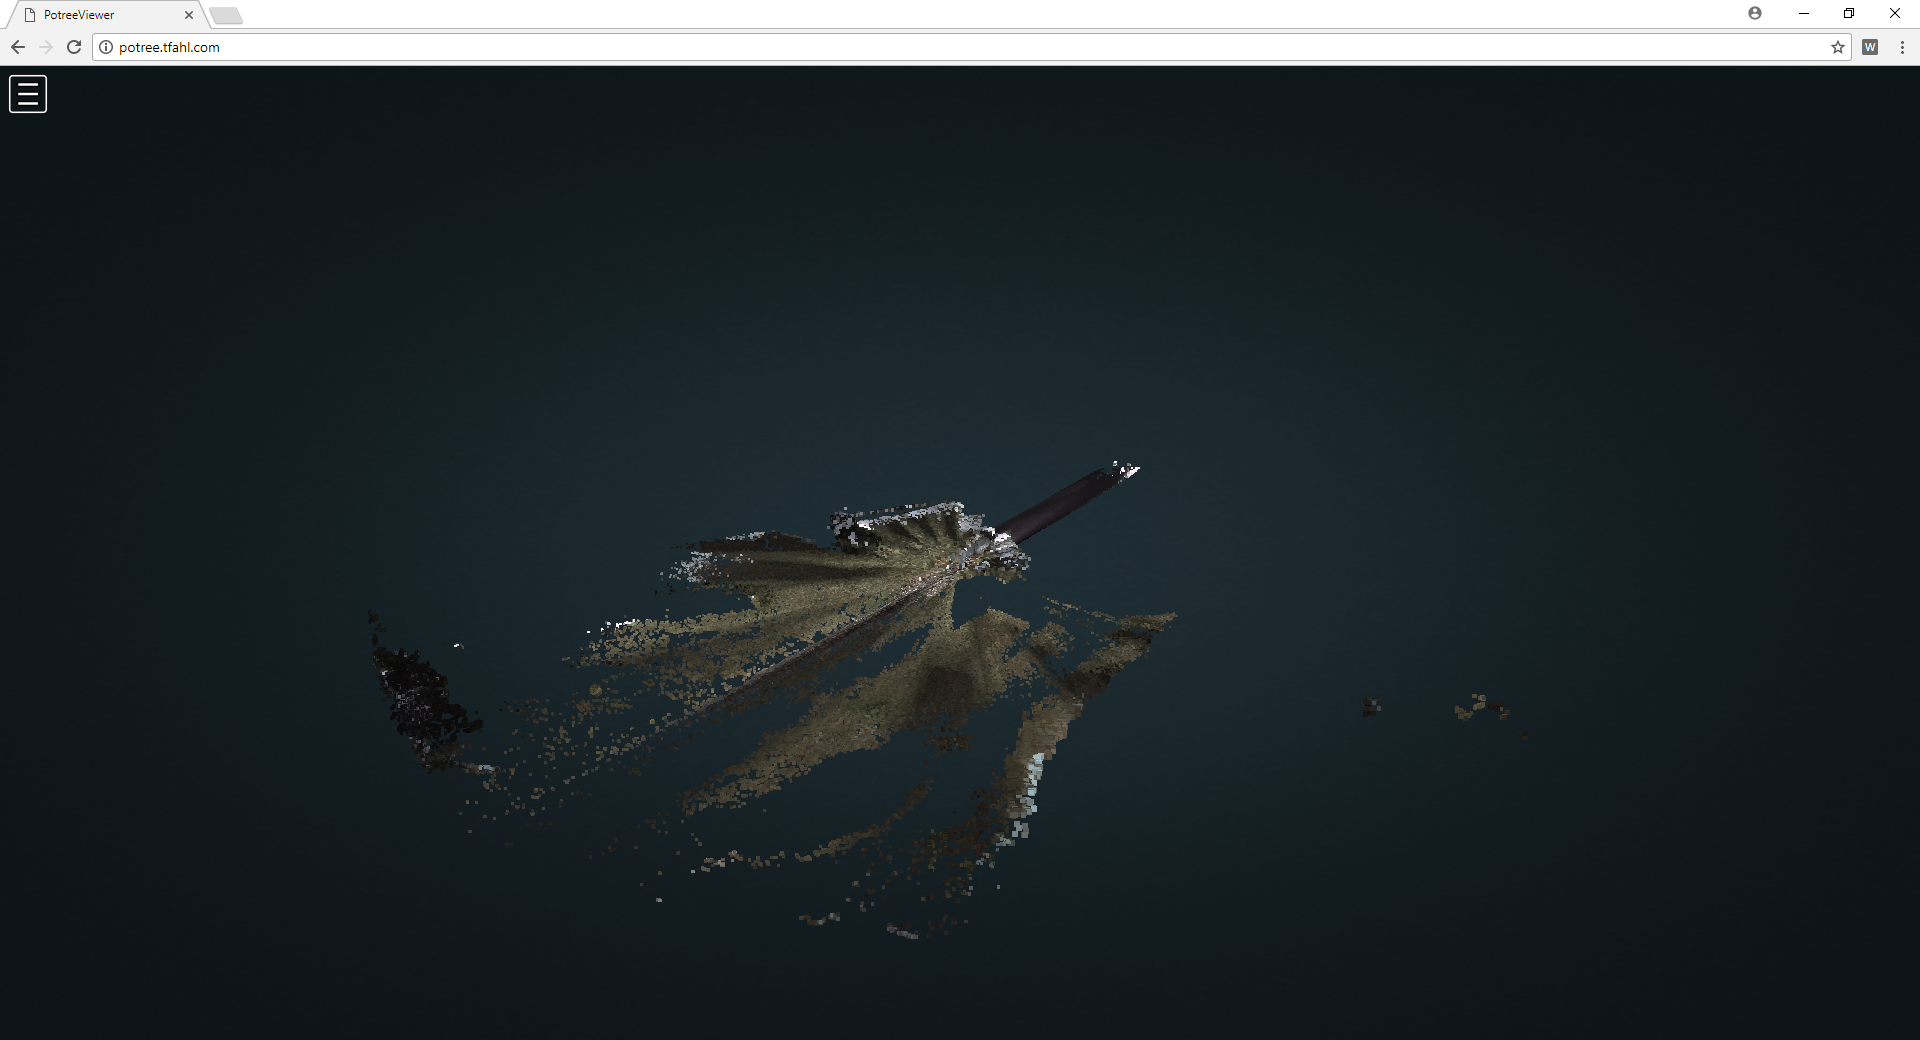
\includegraphics[scale=.25]{NoctVR1}
	\caption{Example of a rendered pointcloud in potree Viewer}
\end{figure}

\begin{figure}[h]
    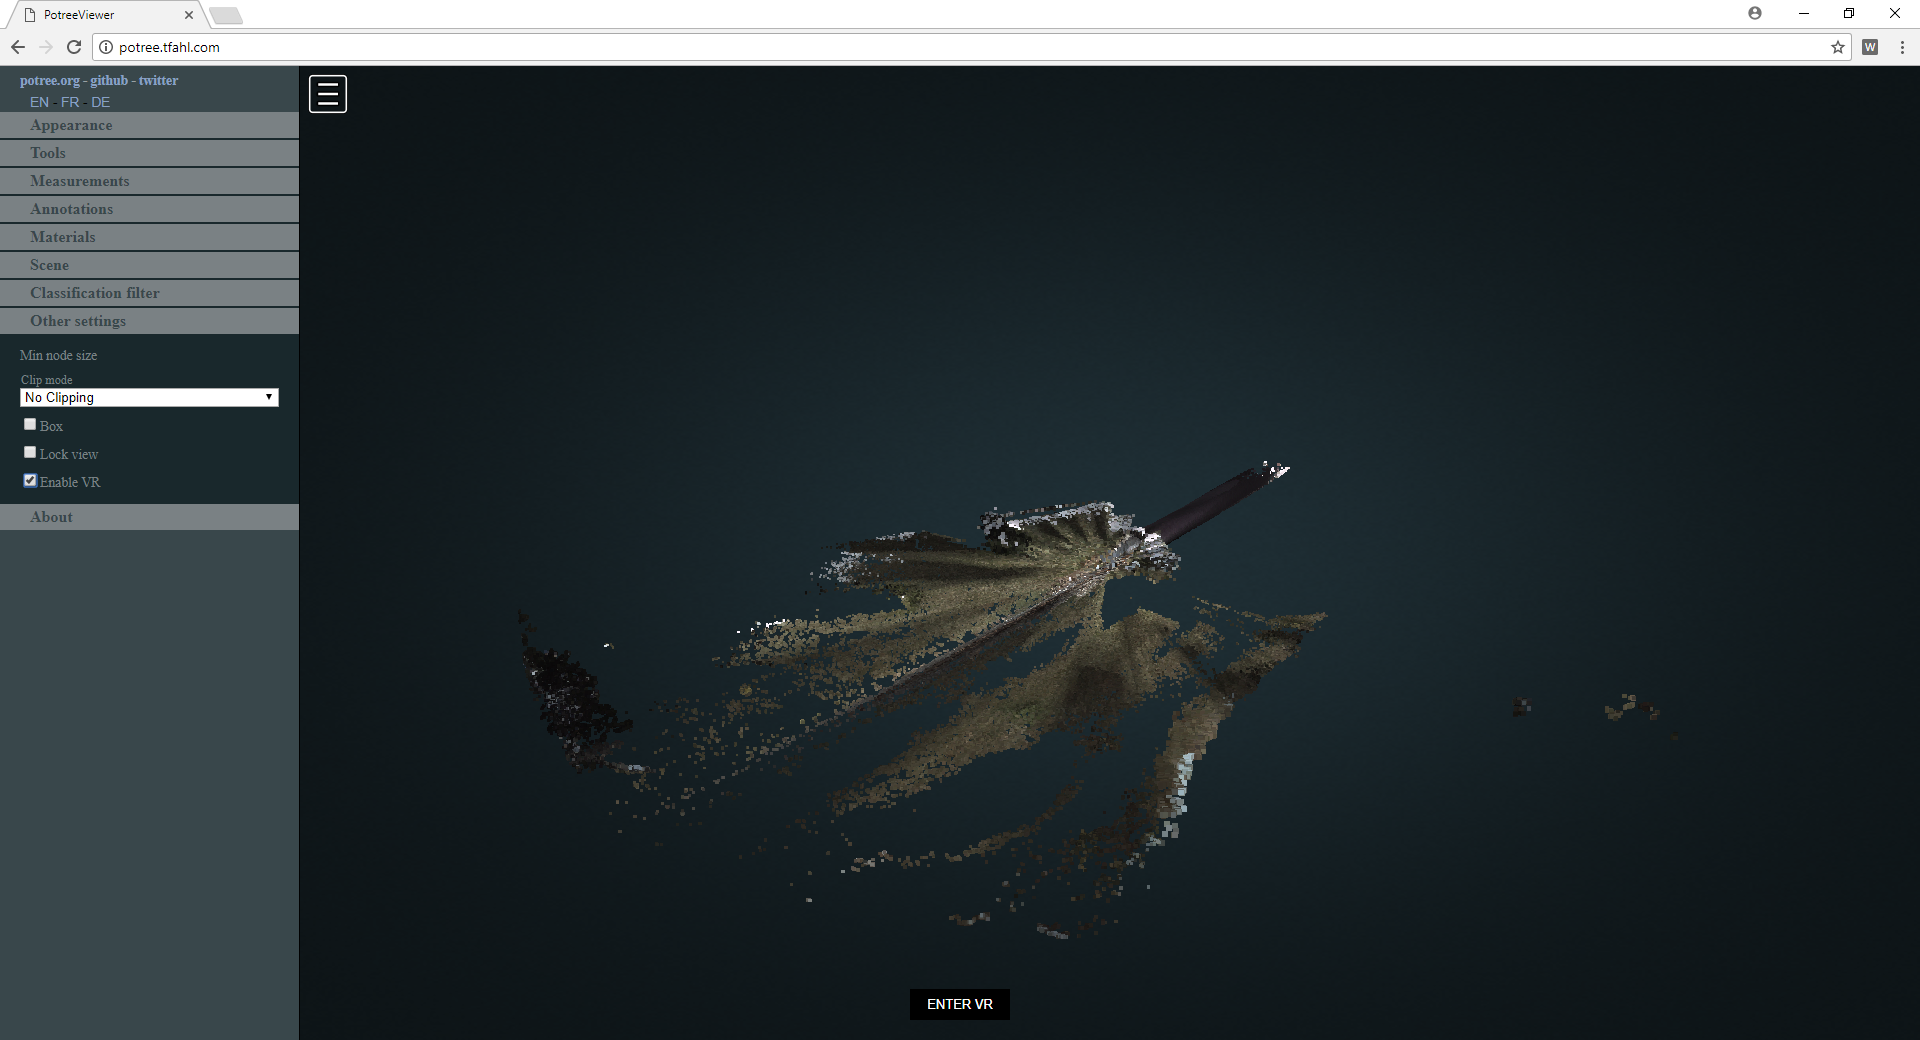
\includegraphics[scale=.25]{NoctVR2}
	\centering
	\caption{potree Viewer with the hamburger menu open, and the Enable VR button visible}
\end{figure}

\begin{figure}[h]
	\centering
    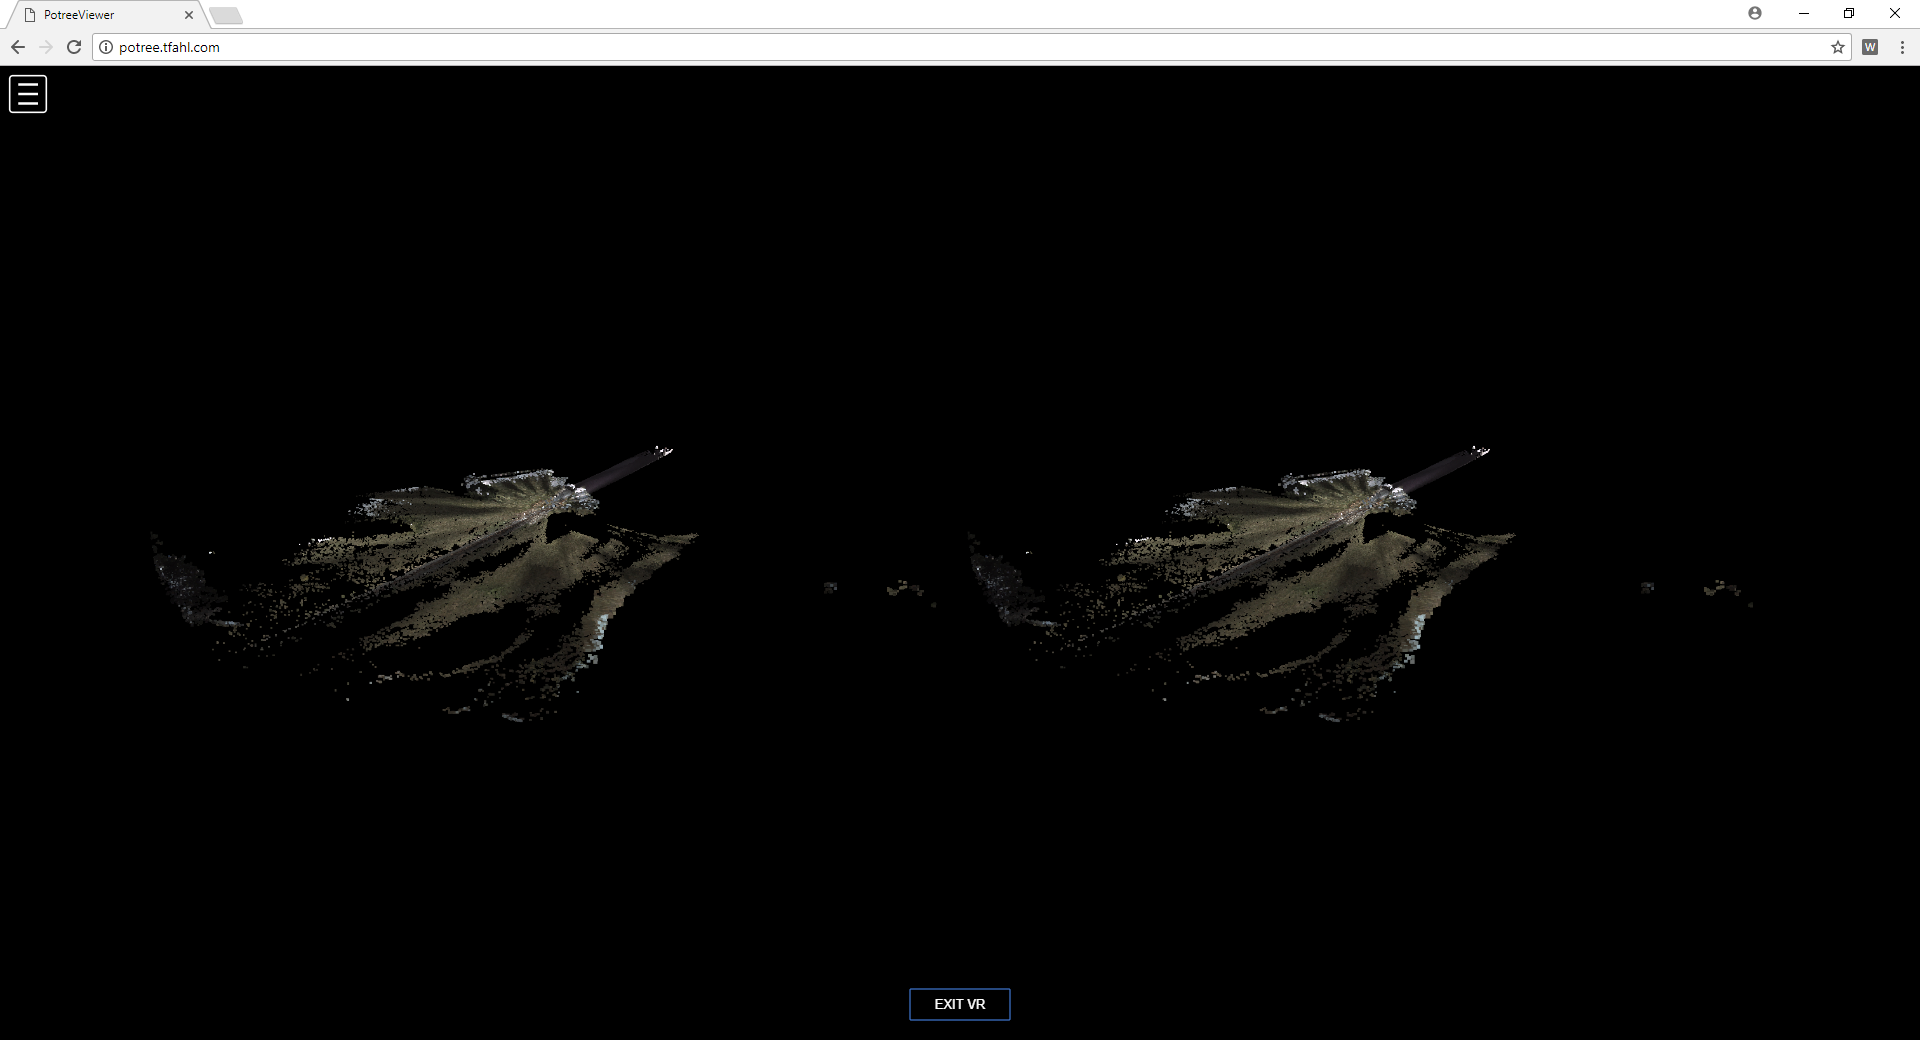
\includegraphics[scale=.25]{NoctVR3}
	\caption{potree Viewer with Noctilucent VR just activated}
\end{figure}

\begin{figure}[h]
	\centering
    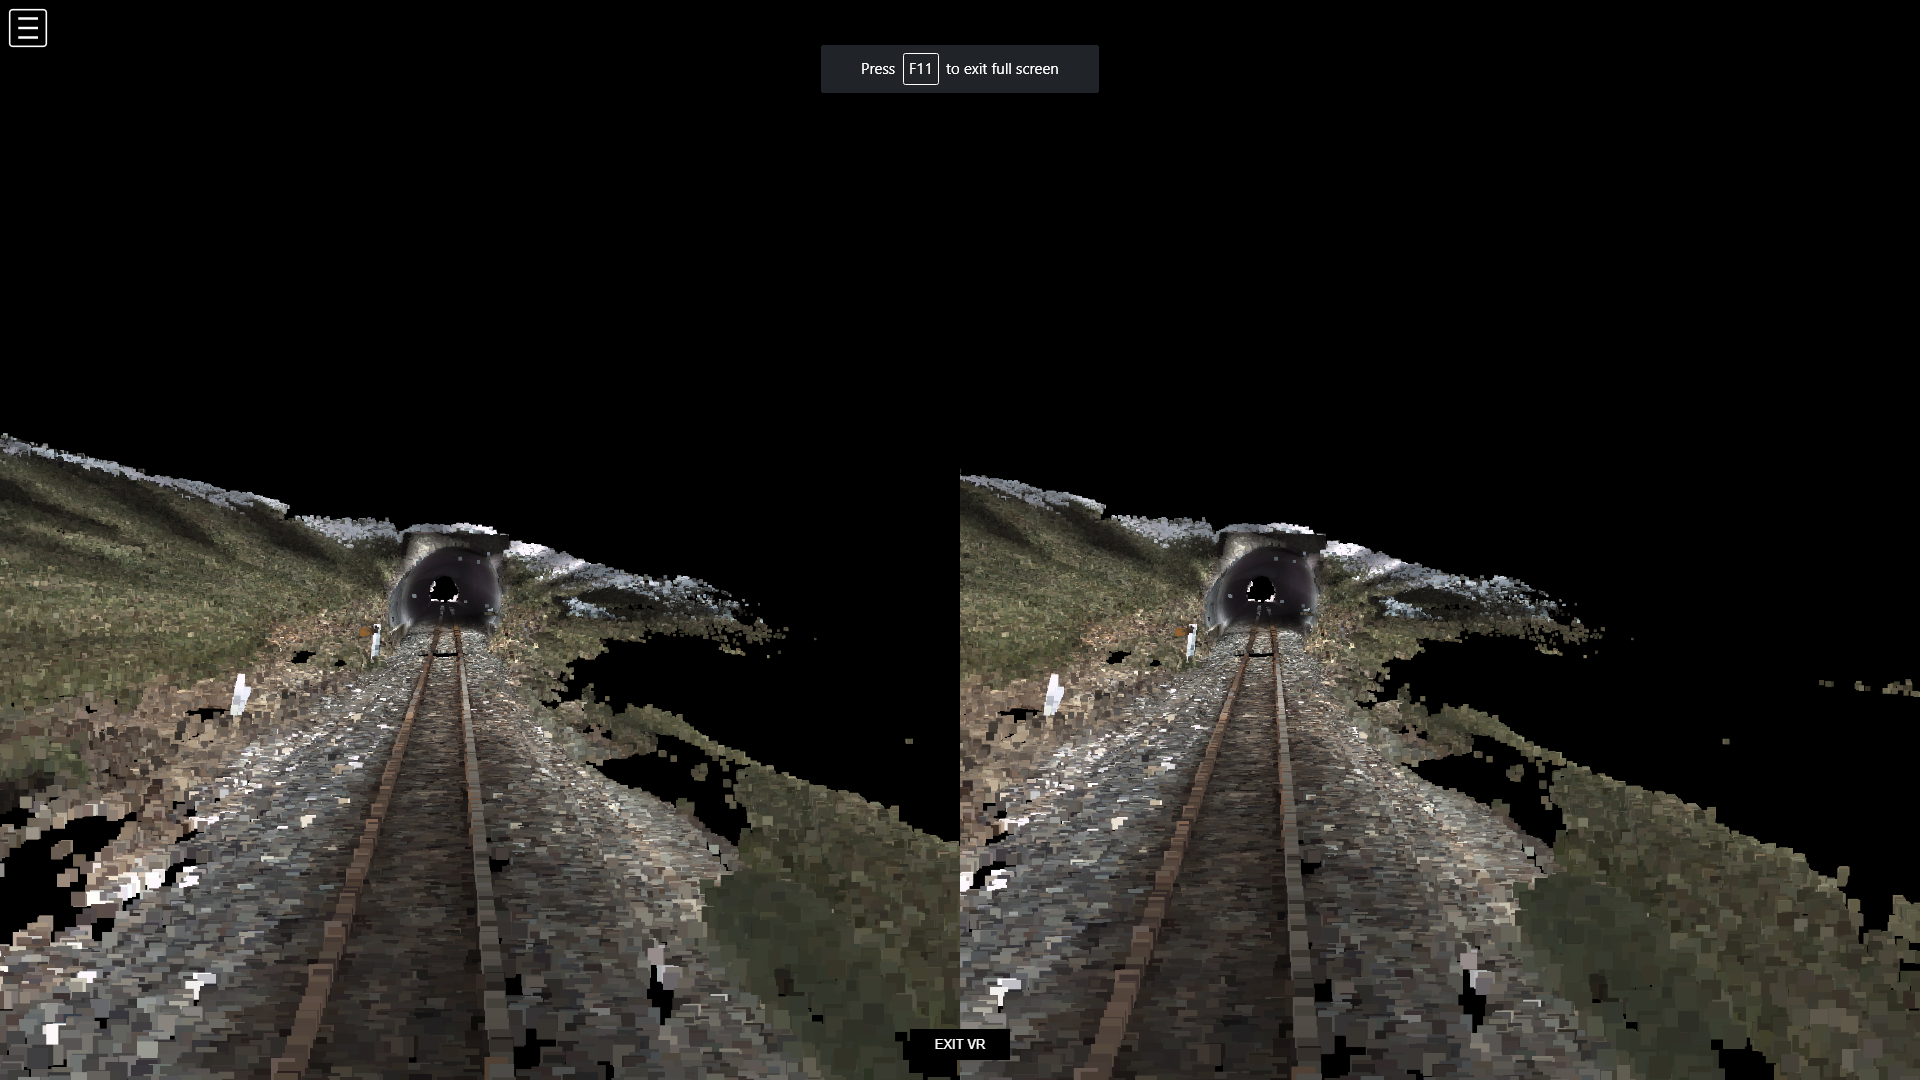
\includegraphics[scale=.25]{NoctVR4}
	\caption{A close-up view of the train tracks with VR-Mode Activated}
\end{figure}

\end{document}
